\documentclass[10pt,a4paper]{scrartcl}
\usepackage[english]{babel} %language
	
\input{../Headerfiles/Packages}
\input{../Headerfiles/Titles}
\input{../Headerfiles/Commands}
\input{../Headerfiles/Mathcolumns}

%-------------------------------------------------------------------
\makeatletter%extension for matrices allows vertical lines
\renewcommand*\env@matrix[1][*\c@MaxMatrixCols c]{%
  \hskip -\arraycolsep
  \let\@ifnextchar\new@ifnextchar
  \array{#1}}
\makeatother

%linespread
\renewcommand{\baselinestretch}{1.3}
%depth of the table of contents
\setcounter{tocdepth}{2}
%-------------------------------------------------------------------

\author{GianAndrea Müller \& Georg Lins, nach der Vorlesung von G. Ochsner}
\title{Summary RT1 \& RT2\vspace{-1ex}}
\begin{document}

\maketitle
\begin{multicols*}{4}
\footnotesize
\tableofcontents
\normalsize
\end{multicols*}

\begin{multicols*}{3}	%divide page into 3 columns
	\parindent 0pt %no indent at the first line of a new paragraph
	\setlength{\columnseprule}{0.5pt}	%column-dividing rule
	\part{RT1}
	\section{Definitions}
	
	\setlength{\columnseprule}{0pt}
	\small
	\begin{multicols*}{2}
	\begin{tabular}{ll@{=}l}
	number of states&n&nx\\
	number of inputs&m&nu\\
	number of outputs&p&ny\\
	\end{tabular}
	\normalsize
	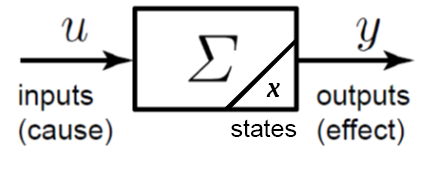
\includegraphics[width=\linewidth]{Signal1}
	\end{multicols*}
	\setlength{\columnseprule}{0.5pt}	
	
	\small
	\begin{tabular}{p{0.45\linewidth}|p{0.45\linewidth}}
	\multicolumn{2}{c}{SISO  /  MIMO}\\
	\hline
	\dahe 1 Eingang / Ausgang & \dahe mehrere Ein- / Ausgänge\\
	\hline
	\hline
	\multicolumn{2}{c}{\vspace{-10pt}}\\
	\multicolumn{2}{c}{dyanmisch  /  statisch}\\
	\hline
	$\frac{d}{dt}y(t)=-\cos(y(t))+u(t)$&$y(t)=\cos(t)u(t)$\\
	enthält Ableitung & enthält keine Ableitung\\
	\hline
	\hline
	\multicolumn{2}{c}{\vspace{-10pt}}\\
	\multicolumn{2}{c}{zeitvariant  /  zeitinvariant}\\
	\hline
	$\frac{d}{dt}y(t)=-\cos(t)y(t)+u(t)$&$\frac{d}{dy}y(t)=-3y(t)+u(t)$\\
	direkte Zeitabhängigkeit& keine direkte Zeitabh.\\
	\hline
	\hline
	\multicolumn{2}{c}{\vspace{-10pt}}\\
	\multicolumn{2}{c}{nicht linear  /  linear}\\
	\hline
	$\frac{d}{dt}y(t)=-y^2(t)+u(t)$&$\frac{d}{dt}y(t)=-y(t)+u(t)$\\
	\hline
	\hline
	\end{tabular}
	\normalsize

	\section{Standard Control System}
	
	\mypic{StandardControlSystem}
	
	\begin{tabular}{l@{ : }ll@{ : }l}
	r&control variable&y&output\\
	F&feedforward&n&noise\\
	C&controller&e&error\\
	P&plant&u&actuating variable\\
	d&disturbance\\		
	\end{tabular}
	
	\subsection*{Function of the controller}
	
	\begin{itemize}
	\compaq
	\item \textbf{Reference tracking:}
	The output $y$ should follow a given input signal $r$.
	\item \textbf{Disturbance rejection:}
	Use feedback to compensate disturbances $d$.
	\item \textbf{Stabilization:}
	Stabilize a system that would naturally deviate from the desired equilibrium. (Inverted pendulum)
	\end{itemize}
		
	\section{System Representation}
	\mypic{Modelling}
	
	\subsection{Modelling}
	\begin{enumerate}
	\compaq
	\item
	Identify the \textbf{system boundaries}.
	\item
	Identify \textbf{relevant reservoirs} and their \textbf{level variables}.
	\item
	\fbox{$\frac{\partial}{\partial t}(\text{reservoir content})=\sum\text{inflows}-\sum\text{outflows}$}
	\end{enumerate}
	
	\begin{align*}
	\frac{d}{dt}z(t)&=f(z(t),v(t))\\
	w(t)&=g(z(t),v(t))
	\end{align*}
	
	\subsection{Normalization}
	Replace the physical variables z(t),v(t) and w(t) by \textbf{normalized variables x(t), u(t) and y(t)}, which have a magnitude of $\approx$1.
	
	$z_i(t)=z_{i,0}\cdot x_i(t),\qquad v(t)=v_0\cdot u(t),\qquad w(t)=w_0\cdot y(t)$
	
	\begin{align*}
	\frac{d}{dt}x(t)&=f_0(x(t),u(t))\\
	y(t)&=g_0(x(t),u(t))
	\end{align*}
	
	\subsection{Linearization}
	
	Linearize the system around an equilibrium point $(x_e,u_e)$, where $\frac{d}{dt}\vec{x}(t)=0$ and $\frac{d}{dt}y(t)=0$.
	
	\begin{alignat*}{4}
	x_i(t)&=x_{i,e}+\delta x_i(t)&\text{ with  }&|\delta x_i(t)|\ll 1,\\
	u(t)&=u_e+\delta u(t)&\text{ with  }&|\delta u(t)|\ll 1,\\
	y(t)&=y_e+\delta y(t)&\text{ with  } &|\delta y(t)|\ll 1
	\end{alignat*}
	
	\begin{alignat*}{3}
	\frac{d}{dt}\delta x(t) &= \frac{\partial f_0}{\partial x}|_{x=x_e,u=u_e}\cdot \delta x(t)&+\frac{\partial f_0}{\partial u}|_{x=x_e,u=u_e}\cdot \delta u(t)\\
	\delta y(t)&=\frac{\partial g_0}{\partial x}|_{x=x_e,u=u_e}\cdot\delta x(t) &+\frac{\partial g_0}{\partial u}|_{x=x_e,u=u_e}\cdot\delta u(t)
	\end{alignat*}
	
	Delays are neglected within the state-space description.
	
	\mypic{NormierungLinearisierung}
	
	\subsection{State-Space Description}
	
	
	\begin{alignat*}{3}
	\frac{d}{dt}x(t)&=A\cdot x(t) &+ b\cdot u(t)\\
	y(t)&=c\cdot x(t) &+d\cdot u(t) 
	\end{alignat*}
	
	
	
	\subsection{I/O Description}
	
	Differential equation connecting the output $y(t)$ directly to the input $u(t)$.
	
	$y^{(n)}(t)+a_{n-1}y^{n-1}+\cdots+a_1y^{(1)}(t)+a_0y(t)=$
	
	$b_mu^{(m)}(t)+\cdots+b_1u^{(1)}(t)+b_0u(t)$
	
	
	
	\subsection{Frobenius Form}
	
	State-space description from I/O description or transfer function.
	
	\importname{$\frac{b_ms^{(m)}+b_{m-1}s^{(m-1)}+\cdots+b_1s+b_0}{s^{(n)}+a_{n-1}s^{(n-1)+\cdots+a_1s+a_0}}$}{Transfer function}
	
	if $m<n$:
	
	\setlength{\tabcolsep}{3pt}
	$\left[\begin{tabular} {c|c} A & b\\ \hline  c & d\end{tabular}\right]$=$\left[\begin{tabular}{cccccc|c}
	0 & 1 & 0 & $\cdots$ & $\cdots$ & 0 & 0\\
	0 & 0 & 1 & 0        & $\cdots$ & 0 & 0\\
	$\vdots$ & $\vdots$ & $\vdots$ & $\vdots$ & $\vdots$ & $\vdots$ & $\vdots$\\
	0 & $\cdots$ & $\cdots$ & $\cdots$ & 0 & 1 & 0\\
	$-a_0$ & $-a_1$ & $\cdots$ & $\cdots$ & $-a_{n-2}$ & $-a_{n-1}$ & 1\\
	\hline
	$b_0$ & $\cdots$ & $b_m$ & 0 & $\cdots$ & 0 & 0 
	\end{tabular}\right]
	$
	
	if $m = n$:
	
	$\left[\begin{tabular} {c|c} A & b\\ \hline  c & d\end{tabular}\right]$=$\left[\begin{tabular}{cccccc|c}
	0 & 1 & 0 & $\cdots$ & $\cdots$ & 0 & 0\\
	0 & 0 & 1 & 0 & $\cdots$ & 0 & 0 \\
	$\vdots$ & $\vdots$ & $\vdots$ & $\vdots$ & $\vdots$ & $\vdots$ & $\vdots$\\
	0 & $\cdots$ & $\cdots$ & $\cdots$ & 0 & 1 & 0\\
	$-a_0$ & $-a_1$ & $\cdots$ & $\cdots$ & $-a_{n-2}$ & $-a_{n-1}$ & 1\\
	\hline
	\multicolumn{2}{c}{$(b_0-b_na_0)$}&$\cdots$&$\cdots$&\multicolumn{2}{c|}{$(b_{n-1}-b_na_{n-1})$}&$b_n$
	\end{tabular}\right]$	

	
	
		
	
	\section{Analysis of Linear Systems}
	
	\subsection{Time domain solution of y(t)}
	
	Given the state-space descritption $\left[\begin{tabular} {c|c} A & b\\ \hline  c & d\end{tabular}\right]$ we can derive:
	
	\begin{center}
	\fbox{
	$y(t)=c\cdot e^{A\cdot t}\cdot x(0)+\int_0^t{c\cdot e^{A(t-\rho)}\cdot b\cdot u(\rho)\cdot d\rho+}d\cdot u(t)$}
	\end{center}
	
	
	
	\subsection{Lyapunov Stability}
	
	\begin{center}
	$\lambda_i$ are the Eigenvalues of A. $\Leftrightarrow\ \det(A-\lambda I)=0$
	\end{center}
	
	\begin{tabular}{p{0.47\linewidth}p{0.47\linewidth}}
	$\Re(\lambda_i)< 0$ & asymptotically stable\\
	$\Re(\lambda_i)\leq 0$ & stable \\
	$\Re(\lambda_i)>0$ & unstable
	\end{tabular}
	
	\subsubsection{Lyapunov's Stability Principle}
	
	\emph{If the linearization of a nonlinear system around an isolated equilibrium point $x_e$ is asymptotically stable (unstable), then this equilibrium is an asymptotically stable (unstable) equilibrium of the nonlinear system as well.}
	
	
	
	\subsection{Block diagram}
	
	We can depict the state space model with a series of integrators in a block diagram.
	
	\setlength{\tabcolsep}{1ex}
	For example $\left[\begin{tabular} {c|c} A & b\\ \hline  c & d\end{tabular}\right]$ = $\left[\begin{tabular}{cccc|c}
	0 & 1 & 0 & 0 & 0\\
	3 & 0 & 0 & 2 & 1\\
	0 & 0 & 0 & 1 & 0\\
	0 & -2 & 0 & 0 & 0\\
	\hline
	1 & 0 & 0 & 0 & 0.5
	\end{tabular}\right]$
	
	\mypic{Blockschaltbild}
	
	
	
	\subsection{Reachability}

	\emph{The possibility to force the system's state x to any location in the state space using the input signal $u$.}
	
	If all points of the state space are reachable, i.e. there exists an input that makes the system reach any point in finite time, the system is \textbf{completly controllable}. Note: complete reachability is prequisite.
	
	n
	
	Reachability condition: $\{A,b\}$ is completly controlable iff 
	\begin{center}
	\fbox{	
	$\mathcal{R}_n=\begin{bmatrix}b&A\cdot b&A^2\cdot b&\cdots&A^{n-1}\cdot b\end{bmatrix}\in\mathbb{R}^{n\times n}$}
	\end{center}
		
	has full rank.
	
	

	\subsubsection{Stabilizability}
	
	An (unstable) system is potentially stabilizable if all uncontrollable state variables are asymptotically stable.
	
	\columnbreak
	
	\subsection{Observability}
	
	\emph{The possibility to reconstruct the initial condition $x(0)$ of the system based only on the output.}
	
	Observability condition: $\{A,c\}$ is completly observable iff 
	\begin{center}
	\fbox{
	$\mathcal{O}_n=\begin{bmatrix}
	c\\
	c\cdot A\\
	\vdots\\
	c\cdot A^{n-1}
	\end{bmatrix}
	\in\mathbb{R}{n\times n}$} has full rank n.
	\end{center}
	
	
	
	\subsubsection{Detectability}
	
	A system is detectable iff all of its unobservable state variables are asymptotically stable.
	
	
	
	\subsection*{Controllability/observability of the nonlinear system}
	
	Linearization completly controllable/observable at equilibrium point $\Rightarrow$ nonlinear System completly (locally) controllable/observable as well.
	
	n	
	
	Linearization \textbf{not} completly controllable/observable $\Rightarrow$ \textbf{no conclusion about the nonlinear system possible!}
	
		
	
	\subsection{State Space Decomposition}
	
	In General the state space can be devided into four subspaces:	
	
	\begin{tabular}{l@{ : }l}
	$RO$&controllable and observable\\
	$\bar{R}O$&not controllable but observable\\
	$R\bar{O}$&controllable but not observable\\
	$\bar{R}\bar{O}$&not controllable and not observable
	\end{tabular}

\mypic{StateSpaceDecomposition}

	
	
	\subsection{Minimal realization}
	
	For every system a coordinate transformation can be found which yields a system of the form:
	
	$\left[\begin{tabular} {c|c} $\tilde{A}$ & $\tilde{b}$\\ \hline  $\tilde{c}$ & d\end{tabular}\right]$=$\left[\begin{tabular}{cccc|c}
	$\tilde{A}_{11}$&$\tilde{A}_{12}$&$\tilde{A}_{13}$&$\tilde{A}_{14}$&$\tilde{b}_1$\\
	0&$\tilde{A}_{22}$&0&$\tilde{A}_{24}$&0\\
	0&0&$\tilde{A}_{33}$&$\tilde{A}_{34}$&$\tilde{b}_3$\\
	0&0&0&$\tilde{A}_{44}$&0\\
	\hline
	0&0&$\tilde{c}_3$&$\tilde{c}_4$&d
	\end{tabular}\right]$
	
	\dahe only state variables that can be controlled by the input and have an influence on the output are accounted for in the minimal realization.
	
	\begin{itemize}
	\compaq
	\item
	Unobservable state variables are negligible. ($\tilde{x}_1,\tilde{x}_2$)
	\item
	Uncontrolable state variables are negligible. ($\tilde{x}_2,\tilde{x}_4$)
	\item
	Note: This way of simplification can \textbf{only be used if matrix A is in triangular form}. Otherwise the alternative procedure is needed!
	\end{itemize}
	
	What remains is the minimal realization: $\{\tilde{A}_{33},\tilde{b}_3,\tilde{c}_3,d\}$
	
	\subsubsection{Alternative procedure}
	
	\begin{enumerate}
	\compaq
	\item
	Derive the transfer function.
	\item
	Use the Frobenius form to find the state space model of the minimal realization.
	\end{enumerate}
	
	
	
	\subsection{Laplace-Transformation}
	
	\subsubsection{Definition}
	
	$\mathcal{L} \{x\}=X(s)=\int_0^\infty{x(t)\cdot e^{-st}dt}$
	
	\subsubsection{Identities}
	\small
	\begin{tabulary}{\linewidth}{L@{  :  }l}
	linearity&$\mathcal{L}\{a\cdot f_1(t)+b\cdot f_2(t)\}=a\cdot F_1(s)+b\cdot F_2(s)$\\
	similarity&$\mathcal{L}\{\frac{1}{a}x(\frac{t}{a})\}=X(s\cdot a)$\\
	shift&$\mathcal{L}\{x(t-T)\}=e^{-T\cdot s}\cdot X(s)$\\
	damping&$\mathcal{L}\{x(t)\cdot e^{a\cdot t}\}=X(s-a)$\\
	derivative t&$\mathcal{L}\{\frac{d}{dt}x(t)\}=s\cdot X(s)-x(0)$\\
	derivative s&$\mathcal{L}\{t\cdot x(t)\}=-\frac{d}{ds}X(s)$\\
	integration t&$\mathcal{L}\{\int_0^t{x(\tau)d\tau}\}=\frac{1}{s}X(s)$\\
	integration s&$\mathcal{L}\{\frac{1}{t}x(t)\}=\int_0^\infty{X(\sigma)d\sigma}$\\
	convolution t&$\mathcal{L}\{x_1(t)*x_2(t)\}=X_1(s)\cdot X_2(s)$\\
	convolution s&$\mathcal{L}\{x_1(t)\cdot x_2(t)\}=X_1(s)*X_2(s)$\\
	initial value&$\lim\limits_{t\rightarrow 0_+}{x(t)}=\lim\limits_{s\rightarrow\infty}{s\cdot X(s)}$\\
	final value&$\lim\limits_{t\rightarrow\infty}{x(t)}=\lim\limits_{s\rightarrow 0_+}{s\cdot X(s)}$
	\end{tabulary}
	\normalsize
	
	\subsubsection{Transform Table}
	
	\begin{tabular}{p{0.45\linewidth}|p{0.45\linewidth}}
	\hline
	$\text{impulse: }\delta(t)$&$1$\\
	$\text{step: }h(t)$&$\frac{1}{s}$\\
	$h(t)\cdot t^n\cdot e^{\pi t}$&$\frac{n!}{(s-\pi)^{n+1}}$\\
	$h(t)\cdot\sin(\omega\cdot t)$&$\frac{\omega}{s^2+\omega^2}$\\
	$h(t)\cdot\cos(\omega\cdot t)$&$\frac{s}{s^2+\omega^2}$\\
	\hline
	\end{tabular}
	
	\subsection{Transfer Function}\label{SisoTF}
	
	\mypic{LaplaceTransformOverview}
	
	\mypic{SystemRepresentation}
	
	\large
	\importable{$\Sigma(s)=c\cdot$&$(sI-A)^{-1}\cdot b+d$\\\vspace{-10pt}&\\&$(sI-A)^{-1}=\frac{\text{Adj}(sI-A)}{\det(sI-A)}$}
	\normalsize
	
	Adj$(A)=C^T$ (transpose of the cofactor matrix)
	
	$C_{ij}=(-1)^{i+j}M_{ij}$
	
	$M_{ij}$ is the determinant of the $\mathcal{R}^{n-1\times n-1}$ Matrix that results form deleting row i and column j.
	
	\subsubsection{For a 2$\times$2 matrix}
	
	\large
	$A=\begin{bmatrix}
	a&b\\
	c&d
	\end{bmatrix}\qquad (A)^{-1}=\frac{1}{\det(A)}\begin{bmatrix}d&-b\\-c&a\end{bmatrix}$
	\normalsize
	
	\subsubsection{Simplification}
	
	If $b$ or $c$ contain zeros:
	
	$c\cdot(sI-A)^{-1}\cdot b=\begin{bmatrix}1&0\end{bmatrix}\cdot\begin{bmatrix}*&x\\ * & *\end{bmatrix}\cdot\begin{bmatrix}0\\2\end{bmatrix}$
	
	in this case only calculate $x$ because all the other matrix components will be multiplied with 0.
	
	\finn
		
	
	\subsection*{Inverse Laplace Transform}
	
	$Y(s)=\frac{\xi(s)}{(s-\pi_1)^{\phi_1}\cdot(s-\pi_2)^{\phi_2}\cdots(s-\pi_p)^{\phi_p}}=\sum\limits_{i=1}^{p}\sum\limits_{k=1}^{\phi_i}\frac{\rho_{i,k}}{(s-\pi_i)^k}$
	
	\finn	
	
	\large
	\begin{center}
	
	\fbox{$\rho_{i,k}=\lim\limits_{s\rightarrow\phi_i}{\frac{1}{(\phi_i-k)!}\left(\frac{d^{(\phi_i-k)}}{ds^{(\phi_i-k)}}\ \left(Y(s)\cdot(s-\pi_i)^{\phi_i}\right)\right)}$}

	\finn	
	
	\fbox{$y(t)=\sum\limits_{i=1}^{p}\sum\limits_{k=1}^{\phi_i}{\frac{\rho_{i,k}}{(k-1)!}\cdot t^{k-1}\cdot e^{\pi_i t}\cdot h(t)}$}
	\end{center}
	\normalsize
	
	\finn	
	
	
	
	\section{Transfer functions}

	$\Sigma(s)=\frac{Y(s)}{U(s)}=\frac{P_m(s)}{P_n(s)}$
	
	\subsection{Poles}
	
	\emph{The poles of the transfer function of a system define its impulse response in the time domain an thereby its inherent dynamics.}
	
	\begin{center}
	\fbox{$\pi_i=\text{ roots of }P_n(s)$}
	\end{center}
	
	\begin{itemize}
	\compaq
	\item
	If the system is a minimal realization $\pi_i$ are equivalent to $\lambda_i$. Otherwise there will be pole-zero cancellations.
	\item
	Poles cannot be changed.
	\end{itemize}
	
	
	
	\subsubsection{BIBO Stability}
	
	\footnotesize(bounded-input-bounded-output)\normalsize
	
	\important{$\int_0^\infty{|\sigma(t)|dt}<\infty\qquad$or$\qquad\Re(\pi_i)<0$}
	 
	\subsubsection{Comparison Lyapunov / BIBO}
	 	 
	 
	\begin{tabular}{p{0.4\linewidth}cp{0.45\linewidth}}
	\hline
	\multicolumn{3}{l}{For a system in minimal realization:}\\
	\hline
	\hline
	\textbf{Lyapunov}&&\textbf{BIBO}\\
	asymptotically stable&$\Leftrightarrow$& stable\\
	stable&$\Rightarrow$&Not stable\\
	unstable&$\Rightarrow$&Not stable\\
	stable or unstable&$\Leftarrow$&Not stable\\
	\hline
	\multicolumn{3}{l}{with uncontrollable or unobservable modes}\\
	\hline
	\hline
	\textbf{Lyapunov}&&\textbf{BIBO}\\
	asymptotically stable&$\Rightarrow$&stable\\
	stable&$\Rightarrow$&?\\
	unstable&$\Rightarrow$&?\\
	stable or unstable&$\Leftarrow$&Not stable\\
	?&$\Leftarrow$&stable
	\end{tabular}
	 
	
	
	\subsection{Zeros}
	
	\emph{The zeros of the transfer function of a system define the dynamics yielding an output of zero.}
	
	\important{$\zeta_i =\text{roots of} P_m(s)$}
	
	\begin{itemize}
	\compaq
	\item
	Zeros can often be shifted by a different sensor configuration.	
	\item
	A zero can reduce the influence of a pole that is close.
	\item
	A zero can lead to over- or undershoot.
	\item 
	If a zero coincides with a pole the cancel out and the order of the system appears to be reduced.
	\end{itemize}
	
	
	
	\subsubsection{Nonminimumphase-Zeros (NMPZ)}
	
	\important{$\Re(\zeta)>0$}
	
	\emph{A system with a NMPZ reacts to an input signal with undershooting.}
	
	\mypic{Minimumphase}
	
	\begin{itemize}
	\compaq
	\item
	The closer a zero is to 0, the more the system oscillates.
	\item
	NMPZ are much more precarious than MPZ. The controller is requiered to "ignore" the undershooting, which makes it slower.
	\item
	The slope of the step answer (at t=0) is 0 iff the transfer function has no zeros.
	
	\end{itemize}
	
	\columnbreak
	
	\subsection{Step Answer}
	
	\subsubsection{Static Gain}
	
	\important{$\Sigma(0)$ represents the static gain of a system.}
	
	\emph{The static gain is the asymptotic value of the step response.}	
	
	$\lim\limits_{t\rightarrow\infty}{y}=\Sigma(0)$
	
	
	
	\section{Frequency Response}
	
	\emph{The idea of the frequency response is to analyze how the system reacts to a harmonic input signal.}
	
	\begin{itemize}
	\compaq
	\item
	If a system is excited with a harmonic input it will produce a harmonic output.
	\item
	The output is transient in the beginning and will reduce to it's steady-state response after some time.
	\item
	Mathematically speaking the steady-state response is the particular solution of the differential equation system. 
	\end{itemize}
	
	\important{$y_\infty(t)=|\Sigma(j\omega)|\cdot\cos\left(\omega t+\angle\Sigma(j\omega)\right)$}
	
	\importable{
	$\Sigma(j\omega)=\frac{a(j\omega)}{b(j\omega)}\qquad|\Sigma(j\omega)|=\frac{|a(j\omega)|}{|b(j\omega)|}$&\\
	$\angle\Sigma(j\omega)=\angle a(j\omega)-\angle b(j\omega)$&
	}
	
	\subsection{Bode Diagram}
	
	\emph{The Bode diagram explicitly shows the amplitude and the phase of the system answer to a harmonic input of a spectrum of frequencies.}
	
	\begin{itemize}
	\item
	The frequency axis is logarithmic.
	\item
	The amplitude is measured in decibel.
	\item
	The phase is measured in degrees.
	\end{itemize}
	
	\important{$|\Sigma(j\omega)|_{dB}=20\cdot\log_{10}|\Sigma(j\omega)|$}
	
	\important{$|\Sigma(j\omega)|=10^{\frac{|\Sigma(j\omega)|_{dB}}{20}}$}
	
	\begin{tabular}{|l|c|c|c|c|c|c|c|c|}
	\hline
	$|\Sigma(j\omega)|$&$0$&$0.01$&$0.1$&$1$&$2$&$5$&$10$&$100$\\
	\hline
	$|\Sigma(j\omega)|_{dB}$&$-\infty$&$-40$&$-20$&$0$&$6.02$&$13.97$&$20$&$40$\\
	\hline
	\end{tabular}
	
	\important{
	$\Sigma=\Sigma_1\cdot\Sigma_2\Leftrightarrow\Sigma_{dB}=\Sigma_{1,dB}+\Sigma_{2,dB}\qquad\frac{1}{\Sigma}=-\Sigma_{dB}$}
	
	
	
	\subsubsection{Rules for drawing the bode diagram}
	
	\begin{enumerate}
	\compaq
	\item
	r, k \dahe slope of the magnitude, phase
	\item
	transfer function as product of standard elements \dahe standard element library
	\item
	graphical addition
	
	\end{enumerate}	
	
	\begin{tabular}{ll}
	\multirow{2}{0.45\linewidth}{\Large$\Sigma(s)=\frac{P_m(s)}{P_n(s)}$\normalsize}&Relative degree: $r=n-m$\\
	&Number of poles at $s=0$ : $k$\\
	\end{tabular}
	
	
	\importable{
	slope$_{\omega\rightarrow 0}=\frac{-k\cdot 20dB}{dec}$&\\
	slope$_{\omega\rightarrow\infty}=\frac{-r\cdot 20dB}{dec}$&\\
	\hline
	for minimumphase system:&\\	
	$\phi_{\omega\rightarrow 0}=\begin{cases}
	-k\cdot \pi/2\\
	-\pi/2-k\cdot \pi/2
	\end{cases}$&\\
	$\phi_{\omega\rightarrow\infty}=r\cdot \pi/2$&	
	}
	
	\begin{tabular}{p{0.29\linewidth}|p{0.29\linewidth}|p{0.29\linewidth}}
	&slope change&phase change\\
	\hline
	pole:&&\\
	\hline
	\hline
	$\pi=a,\ a<0$&$-20$dB/dec&$-\pi/2$\\
	$\pi=a,\ a>0$&$-20$dB/dec&$+\pi/2$\\
	\hline
	zero:&&\\
	\hline
	\hline
	$\zeta=b,\ b<0$&$+20$dB/dec&$+\pi/2$\\
	$\zeta=b,\ b>0$&$+20$dB/dec&$-\pi/2$\\
	\hline
	time delay:&&\\
	\hline
	\hline
	$e^{-sT}$&$0$dB/dec&$-\omega\cdot T $[rad]\\
	\hline
	\end{tabular}	
	
	\subsubsection{Bode's Law}
	
	\importable{
	The gradient of the magnitude plot ($k\cdot 20$dB/dec)&\\
	determines the phase shift ($k\cdot \pi/2$)&.
	}
	
	
	
	\subsection{Nyquist Diagram}
	
	\emph{In Nyquist diagrams the curve $\Sigma(j\omega)$ is plotted in the complex plane, where the real and imaginary parts are used as coordinates.}
	
	\begin{itemize}
	\compaq
	\item
	The frequency does not excplicitly appear in the plot.
	\end{itemize}
	
	\mypic{Nyquist}
	
	
	
	\subsubsection{Rules for drawing the nyquist diagram}
	
	\begin{tabular}{p{0.275\linewidth}|p{0.625\linewidth}}
	&change of $\angle\lim\limits_{\omega\rightarrow\infty}{\Sigma(s)}$ per pole / zero\\
	\hline
	$\pi=a,a<0$&$-\pi/2$\\
	$\pi=a,a>0$&$\pi/2$\\
	\hline
	$\zeta=b,b<0$&$\pi/2$\\
	$\zeta=b,b>0$&$-\pi/2$\\
	\hline
	\end{tabular}
	
	\begin{center}
	\large
	$\Sigma(s)=\frac{b_m\cdot s^m+\cdots +b_1\cdot s + b_0}{s^k\cdot(s^{n-k}+\cdots+a_1\cdot s+a_0)}$
	\normalsize
	\end{center}
	
	\important{$\angle\Sigma(0)=\begin{cases}-k\frac{\pi}{2}&\text{if}(\frac{a_0}{b_0})>0\\
	-\pi-k\frac{\pi}{2}&\text{if}(\frac{b_0}{a_0})<0
	\end{cases}$}
	
	\begin{itemize}
	\compaq
	\item
	If $k>0$ the curve comes from infinity.
	\item
	The plot runs through $n$ quadrants.
	\item
	The angle at 0 ($\angle\lim\limits_{s\rightarrow\infty}{\Sigma(s)}$) is $-r\pi/2$.
	\item
	$\Sigma(s)$ contains a delay $e^{-Ts}$ \dahe curve spirals the origin.
	\end{itemize}
	
	
	
	\subsection{Frequency response \dahe transfer function}
	
	\begin{enumerate}
	\compaq
	\item
	Find r,k,n.
	\item
	Transfer function is a multiplication of different standard elements. \dahe \textbf{standard element library} \dahe find parameters.
	\end{enumerate}
	
	\mypic{FRtoTF}
	
	
	
	\subsection{Uncertainty Representation}
	
	\mypic{Uncertainty}
	
	Fitting an uncertainty bound:
	
	\mypic{Uncertainty2}
	
	\important{$W_2(s)=k\cdot\frac{1+T\cdot s}{1+\alpha\dot T \cdot s},\quad \alpha<0, \quad T =\frac{1}{\omega_2\sqrt{\alpha}}$}
	
	
	
	\section{Feedback systems}
	
	\mypic{ClosedLoop}
	
	\important{$Y(s)=S(s)\cdot\left[D(s)+P(s)W_2(s)\right]+T(s)\cdot\left[R(s)-N(s)\right]$}
	
	
	
	\subsection*{Definitions}
	
	\begin{tabular}{lll}
	Loop gain & $L(s)=C(s)P(s)\quad$&$ e\rightarrow y$\\
	Sensitivity & $S(s)=\frac{1}{1+L(s)}$&$ d\rightarrow y\quad, r\rightarrow e$\\
	Compl. sensitivity & $T(s)=\frac{L(s)}{1+L(s)}$&$r\rightarrow y$\\
	&$D(s)=P(s)S(s)$&$w\rightarrow y$
	\end{tabular}
	
	\importable{
	$|L(s)|\gg 1 \Rightarrow S(s)\approx \frac{1}{L(s)} $& and $ T(s)\approx 1$\\
	$|L(s)|\ll 1 \Rightarrow T(s) \approx L(s) $& and $S(s)\approx 1$
	}
	
	\importable{$S(s)+T(s)=1$ \dahe Disturbance and noise cannot&\\ be completely suppressed simultaneously.&}
	
	
	
	\subsection{Nyquist theorem}
	
	\begin{tabular}{l@{= }l}
	$n_+$&$\#$ of instable poles $(\Re>0)$\\
	$n_0$&$\#$ of poles with $\Re = 0$\\
	$n_c$&$\#$ of encirclements of -1 in the nyquist plot\\
	\end{tabular}
	
	\finn	
	
	\small
	$n_c$ is counted positively in counter-clockwise direction when omega is changed from $-\infty$ to $\infty$.	
	\normalsize	
	
	\finn	
	
	\textbf{The closed-loop system is asymptotically stable iff $\mathbf{n_c=n_0/2+n_+}$}
	
	
	
	\subsection{Robustness measures}	
	
	\mypic{Robustness}
	
	\begin{tabular}{lll}
	$\omega_c$&crossover frequency&$|L(j\omega_c)|=1$\\
	$\phi$&phase margin&$180-\angle L(j\omega_c)$\\
	$\omega_{\gamma}$&&$\Im(L(j\omega_\gamma))=0$\\
	$\gamma$&gain margin&$\frac{1}{\gamma}=|L(j\omega_\gamma)|$\\
	$\mu_{min}$&minimum return difference&$\mu=\min|1+L(j\omega)|$\\
	&&$\mu=\frac{1}{\max(S(j\omega))}$\\
	\end{tabular}
	
	\mypic{RobustNyquist}
	
	
	
	\subsection{Constraints on closed-loop system}
	
	\subsubsection{Modelling uncertainty}
	
	\mypic{Constraints}
	
	Robust stability theorem: $|L(j\omega)\cdot W_2(j\omega)|<\underbrace{|1+L(j\omega)|}_{\text{Distance to -1}}$
	
	Can be written as: $|T(j\omega)<|W_2^{-1}(j\omega)|$
	
	\important{$\rightarrow\omega_c$ must be substantially smaller than $\omega_2$.}
	
	\mypic{UpperBound}
	
	
	
	\subsubsection{Nonminimumphase zeros}
	
	The step response of a system with an NMPZ changes sign. Therefore any controller that will not destabilize the system must \glqq wait\grqq\ until the output reaches the correct sign. This corresponds to a limited bandwidth in the loop gain.
	
	\important{$\rightarrow \omega_c$ must be substantially smaller than $\omega_{\zeta^+}$}
	
	$\omega_{\zeta^+}$ is the frequency of the smallest NMPZ.
	
	
	
	\subsubsection{Delay}
	
	A delay limits the bandwidth of the controller because it has to await new information longer.
	
	\important{$\omega_c$ must be substantially smaller than $\omega_T$}
	
	$\omega_T=\frac{1}{T}$ defined by the delay of the loop gain $e^{-sT}$.
	
	
	
	\subsubsection{Unstable poles}
	
	\important{$\omega_c$ must be substantially larger than $\omega_{\pi^+}$}
	
	$\omega_{\pi^+}$ is the frequency defined by the pole with the largest real part.
	
	
	
	\subsubsection{Summary of limitations}
	
	\footnotesize
	\begin{tabular}{l@{ = }l}
	$\omega_c$&cross-over frequency of the loop gain\\
	$\omega_d$&specified maximum disturbance rejection frequency\\
	$\pi^+$&dominant (\glqq fastest\grqq) unstable pole\\
	$\zeta^+$&dominant (\glqq slowest\grqq) NMPZ\\
	$\omega_T$&frequency defined by the delay of the loop gain\\
	$\omega_2$&frequency beyond which the model uncertainty $>$ 100\%\\
	$\omega_n$&specified minimum noise rejection frequency
	\end{tabular}
	
	\tiny{$\omega_d\rightarrow$ cross-over frequency of $\omega_d$\hfill$\omega_n\rightarrow$ cross-over frequency of $\omega_n$}
	
	\large
	\important{$\omega_c\in\left[\max(10\cdot \omega_d,2\cdot\pi^+),\min\left(\frac{\zeta^+}{2},\frac{\omega_T}{2},\frac{\omega_2}{5},\frac{\omega_n}{10}\right)\right]$}
	\normalsize
	
	\mypic{SummaryLimitations}
	
	
	
	\section{Specifications for feedback control systems}
	
	If it is possible to find a controller that satisfies the limitations mentioned it has to be:
	
	\small
	\begin{itemize}
	\compaq
	\item
	Robust
	\item
	Rejecting disturbances and noise
	\item
	No static error
	\item
	Quick response
	\item
	Small/no overshoot
	\item
	Limited control action
	\end{itemize}
	\normalsize
	
	
	
	\subsection*{Control error}
	
	\mypic{ClosedLoop}
	
	$E(s)=S(s)\cdot\left(R(s)-N(s)-D(s)-P(s)\cdot W(s)\right)$
	
	Static error $e_\infty=\lim\limits_{t\rightarrow\infty}{e(t)}$
	
	
	
	\subsubsection{Static error I}
	
	For $r(t), n(t)$ or $d(t) = h(t)$:
	
	$E(s)=S(s)R(s)=S(s)N(s)=S(s)D(s)$
	
	\important{$\lim\limits_{t\rightarrow\infty}{x(t)}=\lim\limits_{s\rightarrow 0_+}{s\cdot X(s)}$}
	
	$e_\infty=\lim\limits_{t\rightarrow\infty_+}{e(t)}=\lim\limits_{s\rightarrow 0_+}{s\cdot S(s)\frac{1}{s}}=S(0)=\frac{1}{1+L(0)}$
	
	\dahe if $L(0)=\infty$ \dahe $e_\infty = 0$
	
	\important{To have $e_\infty=0$, P(s) or C(s) have to be of type $k\geq 1$}
	
	\columnbreak
	
	\subsubsection{Static error II}
	
	For $w(t) = h(t)$
	
	$E(S)=-P(s)W(s)$
	
	\finn
	
	$\lim\limits_{t\rightarrow\infty}{e(t)}=\lim\limits_{s\rightarrow 0}{-s\cdot S(s)\cdot P(s)\cdot W(s)}=$
	
	$=\lim\limits_{s\rightarrow 0}{-s\cdot\frac{P(s)}{1+P(s)C(s)}\cdot\frac{1}{s}=-\frac{P(0)}{1+P(0)S(0)}}$
	
	\finn	
	
	\dahe if $|C(0)|=\infty$ \dahe $e_\infty=0$
	
	\important{To have $e_\infty=0$ C(s) has to be of type $k\geq 1$}
	
	
	
	\subsection*{Specifications for static error}
	
	\small
	\begin{tabular}{|p{0.2\linewidth}|p{0.33\linewidth}            |p{0.33\linewidth}|}
	\hline
	Input signal & $r(t),d(t),n(t)$&$w(t)$\\
	\hline
	$|e_\infty|\leq e_{max}$&$|\frac{1}{1+L(0)}|\leq e_{max}$&$|\frac{P(0)}{1+P(0)C(0)}|\leq e_{max}$\\
	\hline
	$e_\infty=0$&P(s) \textbf{or} C(s) have to be of type $k\geq 1$&C(s) has to be of type $k\geq 1$\\
	\hline
	\end{tabular}
	\normalsize
	
	\subsection*{Overshoot and rise time}
	
	\mypic{Overshoot}
	\small
	$\delta = \frac{-\ln(\hat{\epsilon})}{\sqrt{\pi^2+\ln^2(\hat{\epsilon})}}$\hfill$\omega_0=(0.14+0.4\cdot\delta)\cdot\frac{2\pi}{t_{90}})$
	
	$\omega_c=\sqrt{\sqrt{4\cdot \delta^4+1}-2\delta^2}\omega_0$\hfill$\phi=\frac{\pi}{2}-\arctan\left(\frac{\sqrt{\sqrt{4\cdot\delta^4+1}-2\cdot\delta^2}}{2\cdot\delta}\right)$
	\normalsize	
	
	\finn

	\dahe Rules of thumb, valid if:$\begin{cases}\delta\in[0.45,1]&\\ \text{for simple loop gains}&\\ \text{(no NMPZ or instable poles)}&\end{cases}$
	\importable{
	$\omega_c=\frac{1.7}{t_{90}}$&$t_90=\frac{1.7}{\omega_c}$\\
	$\phi=71^\circ-117^\circ \cdot\hat{\epsilon}\qquad$&$\hat{\epsilon}=\frac{71^\circ-\phi}{117^\circ}$
	}	
	
	
	
	\subsection*{Peaking limitations}
	\footnotesize
	\begin{tabular}{p{0.47\linewidth}p{0.43\linewidth}}
	Small S(s):
	\begin{itemize}
	\compaq
	\item good disturbance rejection
	\item good reference tracking
	\end{itemize}	
	&
	Small T(s):
	\begin{itemize}
	\compaq
	\item good noise rejection
	\item good robustness against modelling errors
	\end{itemize}
	\normalsize
	\end{tabular}
	
	Limit peaking of S(s) and T(s) around $\omega_c$:
	
	\important{$||S||_\infty<S_{max},\quad ||T||_\infty<T_{max},\quad S_{max},T_{max}>1$}
	
	\mypic{PeakingLimitations}
	
	$||S||_\infty<S_{max}\Leftrightarrow L(j\omega)\not\in\left\{|1+z|\leq\frac{1}{S_{max}}\mid z\in \mathbb{C}\right\}$
	
	The loop gain must not enter a circle centered in the point -1 with radius $S_{max}^{-1}$.
	
	\finn
	
	$||T||_\infty<T_{max}\Leftrightarrow L(j\omega)\not\in\left\{\left|\frac{T^2_{max}}{T^2_{max}-1}+z\right|\leq\frac{T_{max}}{T^2_{max}-1}|z\in\mathbb{C}\right\}$
	
	The loop gain must not enter a circle centered in the point $-T^2_{max}/(T^2_{max}-1)$ with radius $T_{max}/(T_{max}^2-1)$ (Apolonius circle). 
	If $T_{max}=1$, the Apolonius circle approaches a straight line, thus $L(j\omega)$ may not enter the left half-plane defined by this line. 
	
	
	
	\section{Controler synthesis}
	
	\subsection{PID Controller}
	
	\mypic{PID}
	
	\textbf{P}roportional
	\begin{itemize}
	\compaq
	\item
	Control action proportional to control error.
	\item
	Fast reduction of control error but static error may result.
	\end{itemize}
	
	\textbf{I}ntegral
	\begin{itemize}
	\compaq
	\item
	Control action proportional to integral over the error in time.
	\item
	Slow but complete reduction of the error.
	\item
	Introduces large overshoot.
	\end{itemize}
	
	\textbf{D}erivative
	\begin{itemize}
	\compaq
	\item
	Control action is proportional to change of the error.
	\item
	$u_D(t)\propto \frac{\partial}{\partial t} e(t) = \frac{\partial }{\partial t} r(t) - \frac{\partial}{\partial t} y(t)$
	
	\finn	
	
	fast change of $r(t)$ \dahe \glqq acceleration\grqq
	
	fast change of $y(t)$ \dahe \glqq deceleration\grqq or damping
	\end{itemize}
	
	\mypic{RollOff}
	
	\important{$C_{PID}=k_p\cdot\left[1+\frac{1}{s\cdot T_i}+s\cdot T_d\right]\cdot\frac{1}{(s\tau+1)^2}$}
	
	The roll-off term $\left(\frac{1}{(s\tau+1)^2}\right)$ prevents an infinitely increasing gain for higher frequencies.
	
	
	
	\subsection{Ziegler and Nichols}
	
	\emph{Usable when measured data is available.}
	
	\begin{enumerate}
	\compaq
	\item
	Set $T_i=\infty$ and $T_d, \tau = 0$.
	\item	
	Increase the gain $k_p$ until the loop reaches a steady-state oscillation.
	\item
	\dahe $k_p^*=\frac{1}{|P(j\omega^*)|}\qquad L(j\omega^*)=-1+0\cdot j \qquad \angle L(j\omega^*)=-\pi$
	\end{enumerate}
	
	\begin{center}
	\begin{tabular}{|p{0.2\linewidth}p{0.2\linewidth}p{0.2\linewidth}p{0.2\linewidth}|}
	\hline
	type & $k_p$ & $T_i$ & $T_d$\\
	P	&	$0.5\cdot k_p^*$ & $\infty$ & $0$\\
	PI	&	$0.45\cdot k_p^*$ & $0.85\cdot T^*$ & 0\\
	PD 	&	$0.55\cdot k_p^*$ & $\infty$	&	$0.15\cdot T^*$\\
	PID	&	$0.6\cdot k_p^*$ & $0.5\cdot T^*$& $0.125\cdot T^*$\\
	\hline
	\end{tabular}
	\end{center}
	
	
	
	\subsection{Lead/Lag}
	
	\important{$C(s)=\frac{T\cdot s +1}{\alpha\cdot T \cdot s +1}$}
	
	\mypic{LeadLag}
	
	
	
	\part{RT2}
	
	\subsection{Plant inversion}
	
	If the behaviour of a system is known very well, in theory $C(s)$ can be written as follows:
	
	\finn
	
	\fbox{$C(s)=P^{-1}(s) \Rightarrow L(s)=1$} which would be a perfect controler.
	
	Alternatively one can define a desired loop gain $L_{des}(s)$:
	
	\fbox{$C(s)=L_{des}(s)\cdot P^{-1}(s)\Rightarrow L(s)=L_{des}(s)$} 
	
	\finn	
	
	\textbf{Problems:}
	\begin{itemize}
	\compaq
	\item
	The plant $P(s)$ is causal but $P^{-1}(s)$ is not. Therefore a controler $C(s)=P^{-1}(s)$ cannot be built.
	
	Solution: Add a roll-off term: $\frac{1}{(\tau \cdot s+1)^k}$
	\item
	If the plan has NMPZ or unstable poles plant inversion is not possible.
	\item
	If the plan has NMPZ it is impossible to eliminate the undershooting completely.
	\end{itemize}	
	
	
	
	\subsubsection{Optimal loop gain}
	
	\important{$L_{des}=\frac{1}{T_i\cdot s}\cdot\frac{1}{(\tau\cdot s+1)}$}
	
	\begin{itemize}
	\compaq
	\item
	Integrator eliminates static error.
	\item
	The magnitude should decrease faster in order to improve performance. A second integrator would result in a unstable system (directly passing through -1). Therefore a pole is introduced.
	\item
	Resulting is a well performing and stable system, \textbf{given that the plant is simple, minimum phase and stable}.
	\end{itemize}
	
	\mypic{PlantInversion}
	
	This design allows for the crossover frequency to be chosen freely. For example, the model uncertainty poses an upper limit to the bandwidth, therefore:
	
	\important{$\omega_{c,des}=\frac{\omega_2}{5}\Rightarrow T_i=\frac{1}{\omega_{c,des}}$}
	
	In order for the system to be stable the phase drop induced by the pole should be after the crossover frequency where $|L(s)|\ll 1$. Thus:
	
	\important{$\tau = \frac{T_i}{2}$}
	
		
	
	\subsection{Loop shaping}
	
	Goals revised:

	\begin{itemize}
	\compaq
	\item
	High amplification at low frequencies for \textbf{disturbance rejection}.
	\item
	Low amplification at high frequencies for \textbf{noise attenuation}.
	\end{itemize}
	
	\begin{center}
	\begin{tabular}{l@{$\quad$}l}
	\textbf{system:} & \textbf{idea:}\\
	simple & plant inversion\\
	\hline
	NMP	&	plant inversion impossible\\
	&small crossover frequency ($\omega_c \overset{!}{<}\zeta^+$)\\
	\hline
	unstable & plant inversion impossible\\
	&use nyquist theorem\\
	\end{tabular}
	\end{center}
	
	\subsubsection{Higher cross-over frequency $\omega_c$}
	
	\begin{itemize}
	\compaq
	\item
	faster
	\item
	nominal system stays robust
	\item
	system with uncertainty gets less robust
	\item
	more noise
	\end{itemize}
	
	
	
	\section{Predictive control}
	
	If \fbox{$T/(T+\tau)>0.3$} \dahe predictive controller.
	
	\note{T = delay $\qquad\tau$ = time constant}
	
	Andvantage: 
	\begin{itemize}	
	\compaq
	\item
	Controller can access non-delayed output.
	\item
	Delay introduces big phase drop which prevents a high bandwidth \dahe slow. A predictor offers a higher bandwidth!
	\end{itemize}
	
	Limits:
	\begin{itemize}
	\compaq
	\item
	Prediction allows a controller design with much less phase drop.
	\item
	The delay cannot be removed. Every transfer function is affected by the same delay as the plant!
	\end{itemize}
	
	Prerequisites:
	\begin{itemize}
	\compaq
	\item
	Plant must be \textbf{asymptotically stable}.
	\item
	A \textbf{good model} of the plant must be available.
	\end{itemize}
	
	\subsubsection{Smith predictor}
	
	\mypic{SmithPredictor}
	
	\mypic{SmithPredictor2}
	
	\columnbreak
	
	\begin{tabular}{l@{ = }p{0.4\linewidth}l@{ = }p{0.45\linewidth}}
	$C(s)$&$\frac{C_r}{1+P_rC_r-P_rC_re^{-sT}}$&$L(s)$&$\frac{C_rP_re^{-sT}}{1+P_rC_r-P_rC_re^{-sT}}$\\
	$S(s)$&$\frac{1+P_rC_r-P_rC_re^{-sT}}{1+P_rC_r}$&$T(s)$&$\frac{C_rP_re^{-sT}}{1+P_rC_r}$
	\end{tabular}
	
	Idea: Use a linear Model of the plant $\hat{P}_r(s)$ that grants access to the non-delayed plant output $\hat{y}_r(t)$.
	
	The feedback signal is the difference between $y(t)$ and $\hat{y}_r(t)$.
	
	\finn	
	
	\begin{minipage}{0.5\linewidth}
	\small
	\begin{itemize}
	\compaq
	\item
	fast
	\item
	robust
	\item
	implementation difficult
	\item
	analysis is difficult
	\item
	problems arise from modelling errors
	\end{itemize}
	\normalsize
	\end{minipage}
	\hfill
	\begin{minipage}{0.4\linewidth}
	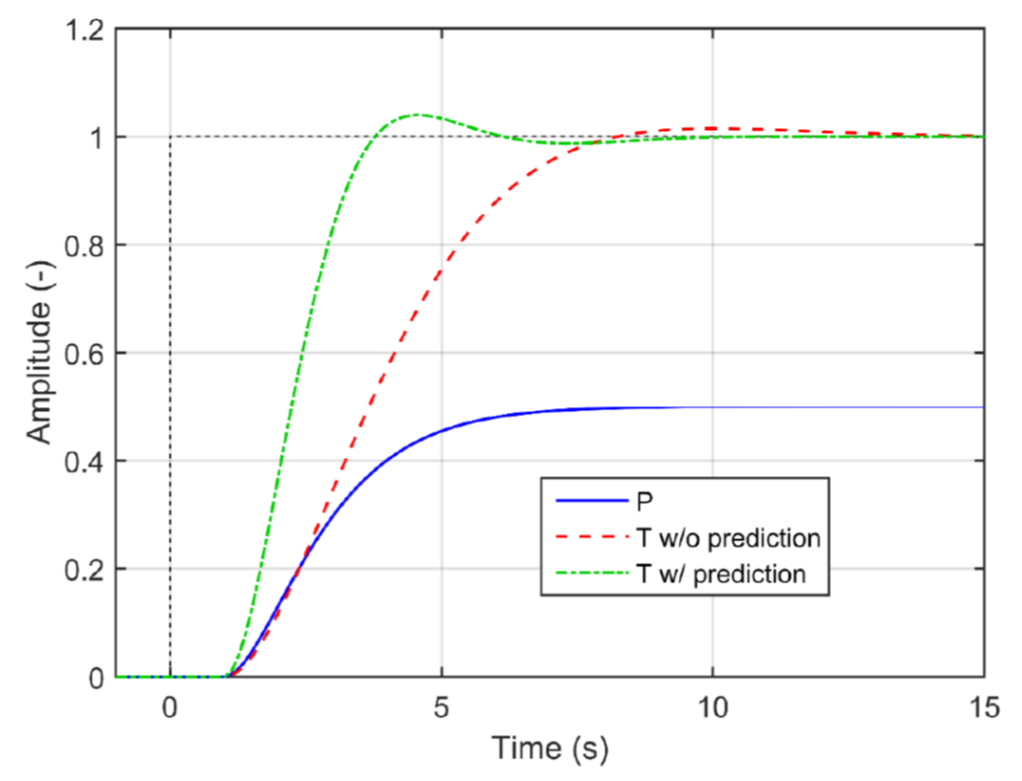
\includegraphics[angle=90,origin=c,width=\textwidth]{SmithResults}
	\end{minipage}
	
	
	
	\section{Robust performance}
	
	\subsection*{Robust nyquist}
	
	The robust nyquist theorem can be interpreted as an upper bound for $T(s)=\frac{L(s)}{1+L(s)}$:
	
	\mimportant{$|T(j\omega)|\cdot|W_2(j\omega)|<1\ \forall\  \omega \in[0,\infty]$\\ or \\$||T(s)\cdot W_2(s)||_\infty<1$\\ or \\$|T(j\omega)|<|W_2^{-1}(j\omega)|$}
	
	\mypic{UpperBoundComplementary}	
	
	\subsection*{Nominal performance}
	
	$S(s)=\frac{1}{1+L(s)}$ is the transfer function from $r\rightarrow e$ and $d\rightarrow y$.
	
	$W_1$ specifies the performance of the controller for the whole frequency-range. How much smaller than 1 should S(s) be? ($W_1(s)$ as an upper bound for $S(s)$). Is defined beforehand as a specification.
	
	\dahe Small sensitivity = good performance.
	
	\mimportant{$|S(j\omega)|\cdot|W_1(j\omega)|<1\ \forall\ \omega\in[0,\infty]$\\ or \\$||S(s)\cdot W_1(s)||_\infty <1$\\or\\$|S(j\omega)|<|W_1^{-1}(j\omega)|$}
	
	\mypic{UpperBoundSensitivity}
	
	\subsection*{Robust performance}
	
	Robust performance represents a combination of the conditions above. If a system is robust it works not only in the academic case but also when subjected to uncertainty and noise.
	
	\important{$|S(j\omega)|\cdot|W_1(j\omega)|+|T(j\omega)|\cdot|W_2(j\omega)|<1\ \forall\ \omega\in[0,\infty]$}
	
	\important{$||S(s)\cdot W_1(s)+T(s)\cdot W_2(s)||_\infty<1$}
	
	\important{$|1+L(s)|<|W_1(s)|+|L(s)\cdot W_2(s)|$}
	
	\begin{center}
	\begin{tabular}{|lll|}
	\hline
	$\omega\rightarrow\infty$&$\quad$:$\quad$&$|L(j\omega)|<\frac{1-|W_1(j\omega)|}{|W_2(j\omega)|}$\\
	$\omega\rightarrow 0$&$\quad$:$\quad$&$|L(j\omega)|>\frac{|W_1(j\omega)|}{1-|W_2(j\omega)|}$\\
	\hline
	\end{tabular}	
	\end{center}	
	
	\mypic{RobustPerformanceBode}
	
	\mypic{RobustPerformance}

	\begin{itemize}
	\compaq
	\item
	The two circles should not touch.
	\item
	$S(s)<W_1^{-1}$ \&\& $T(s)<W_2^{-1}$ no sufficient condition!
	\item
	$W_2\cdot T+W_1\cdot S$ should be below $\SI{0}{\decibel}$.
	\end{itemize}

	\section{Cascaded control}
	
	\mypic{CascadedControl}
	
	\begin{itemize}
	\compaq
	\item
	System with differently dynamic states.
	\item
	Use the faster state variable to build a inner loop with a maximum bandwidth (fast). (Proportional and derivative action)
	\item
	Inner loop represents the new plant for the outer loop.
	\item
	Outer loop, using the slower state variable, designed towards accuracy, including an integrator. 
	\end{itemize}
	
	\section{Setpoint weighting}
	
	\mypic{SetpointWeighting}
	
	\begin{itemize}
	\compaq
	\item Only r is weighted \dahe y is always fed back, even if $a,b,c = 0$.
	\item Setpointweighting only influences the tracking behaviour but not the loop gain. \textbf{Stability \& Robustness are not affected!}
	\item a regulates disturbance rejection.
	\item b regulates reference tracking. 
	\end{itemize}
	
	If disturbances are small compared to reference changes and the actuator is limiting \dahe $0<a<1,\ b=1,\ c=0$.
	
	\begin{itemize}
	\compaq
	\item $0<a<1$ \dahe big reference changes are not weighted as much.
	\item b has to be $=1$, otherwise the integrator would produce a static error.
	\item If $c=0$ only the damping aspect depending on y is used. Steps in r are not influencing the controler ($\frac{\partial}{\partial t}$ for a step is infinite).
	\end{itemize}
	
	\section{Feed forward}
	
	Generalises the idea of using different controlers for reference tracking and disturbance rejection.
	
	\mypic{FeedForward}
	
	\begin{itemize}
	\compaq
	\item
	Improving reference tracking in spite of noise or a fast phase drop of the plant.
	\item
	No feedback
	\item
	Has no influence on the stability of the closed loop.
	\item
	With $F=P^{-1}$ perfect reference tracking is possible. $(y=r)^\ast$
	\item
	Static feed forward \dahe P-controller.
	\item
	Dynamic feed forward \dahe define a desired transfer function $r\rightarrow y$ and derive F.
	\end{itemize}
	
	\mypic{StaticFeedForward}
	
	\note{first linearised, then normalised}
	
	\subsubsection*{Desired transfer function $T_{FF}$}
	
	$T_{FF}=F\cdot P\cdot \frac{1}{1+C\cdot P}+\frac{C\cdot P}{1+C\cdot P}\Rightarrow F\cdot P\cdot S_{fb}+T_{fb}$
	
	\note{$T_{fb},S_{fb}$ transfer functions of the feedback loop
	
	\hlcyan{$S_{fb}\equiv T_{FF}$}}
	
	\subsubsection*{$^\ast$Why $F=P^{-1}$?}
	
	$Y=(P(s)\cdot F(s)\cdot S(s)+T(s))\cdot R$ 
	
	\dahe choose $F=P^{-1}$ \dahe $Y=(S(s)+T(s))\cdot R \Rightarrow Y=R$.
	
	\section{Anti reset-windup}
	
	\subsection*{Actuator saturation}
	
	\mypic{ActuatorSaturation}
	
	$\bar{u}(t)=\begin{cases}u_{max}& \text{if }u(t)>u_{max}\\
	u(t)&else\\
	u_{min}&\text{if }u(t)<u_{min}\end{cases}$
	
	\subsection*{Reset/Integrator windup}
	
	If the actuator is at its saturation the delivered output is constant, thus the control loop is not closed anymore. At the same time the integrator accumulates the corresponding error and continues to push the actuator towards saturation.
	
	\subsection*{Solution}
	
	\mypic{AntiResetWindup}
	
	We include an actuator model in the controller which produces a nonzero output $q(t)$ as soon as the primary controller output differs from the actuator output. In other words as soon as the actuator is saturated. At this point the static gain $k_{ARW}$ prevents the integrator from filling up.	

	\columnbreak
	
	\section{Discrete-time systems}
	
	\begin{tabular}{l@{\dahe}l}
	continuous system&differential equation\\
	discrete system&difference equation
	\end{tabular}
	
	\subsection*{Continuous-time controller}
	
	Transfer functions can be implemented using resistors, capacitors, inductors and operational amplifiers. Effective and fast but expensive and difficult to adjust/debug.
	
	\subsection*{Implementation on microprocessors}
	
	\mypic{DiscreteController}
	
	\note{\hlcyan{See next subsection if the reference is available in digital form.}}
	
	\small
	\begin{tabular}{lll}
	&Name&Task\\
	AAF&Anti-aliasing-filter& (see Aliasing)\\
	ADC&Analog-to-digital-converter&sampling\\
	$\mu$P&microprocessor&contains $C(z)$\\
	DAC&Digital-to-analog-converter & zero order hold
	\end{tabular}
	\normalsize
	
	\note{analog-to-digital \dahe continuous-to-discrete time}	
	
	\finn
	
	Drawback: The zero order hold (applied by DAC), i.e. keeping the output voltage constant over the sampling time introduces a delay of $T/2$.	
	
	\mypic{DiscreteControlSoftware}
	
	\subsection*{Digital reference}
	
	\mypic{DigitalReference}
	
	\subsection*{Lyapunov stability}
	
	\mypic{DiscreteLyapunov}
	
	\subsection*{Sampling}
	
	\mypic{DiscreteADC}
	
	\importname{Sampling frequency}{$F_s=\frac{1}{T}\geq 10 \cdot f_c = 10\cdot\frac{\omega_c}{2\cdot\pi}$}
	
	\note{$\frac{F}{2}$ (Nyquist frequency) is the limit \dahe for security reasons $F_s\geq 10\cdot f_c$}
	
	\finn	
	
	A discrete-time signal with a sampling frequency $F_s$ has no frequency content above $\frac{F_s}{2}$. If the continuous-time signal contains frequencies above $\frac{F_s}{2}$ \textbf{aliasing} occurs.
	
	\subsection*{Aliasing and AAF}
	
	\mypic{Aliasing}
	
	The anti-aliasing filter must be analog, in order to remove high frequency signals before sampling. Practically this is a low-pass filter. \textbf{Always needed to attenuate noise (has high frequency)!}
	
	\subsection*{Controller discretization / Emulation}
	
	PI-controller:
	
	\begin{tabular}{l@{ : }l}
	frequency domain& $U(s)=k_p\left[1+\frac{1}{T_i\cdot s}\right]\cdot E(s)$\\
	time domain&$u(t)=k_p\left[e(t)+\frac{1}{T_i}\cdot\int_0^t{e(\tau)d\tau}\right]$
	\end{tabular}
	
	To implement an I-part in a discrete controller we need to perform numerical integration:
	
	\important{$q(k\cdot T)=\int_0^{k\cdot T}{e(\tau)d\tau}\overset{\text{for example}}{\approx}\sum\limits_{i=0}^{k-1}{e(i\cdot T)}\cdot T$}
	
	\mypic{NumericalIntegration}
	
	\subsubsection{Euler forward}
	
	Discrete-time formulation of the PI-controller:

	$u(k\cdot t)=k_p\cdot\left[ e(k\cdot T)+\frac{1}{T_i}\cdot q(k\cdot T)\right]$
	
	$q(k\cdot T + T)=q(k\cdot T)+e(k\cdot T)\cdot T$
	
	\begin{itemize}
	\compaq
	\item
	$x(k)$ denotes variable x at time $k\cdot T$.
	\item
	The operator z denotes a forward shift by one sampling interval. $z\cdot x(k)=x(k+1)$.
	\end{itemize}
	
	\subsubsection*{Derivation of the euler forward rule}
	
	$u(k)=k_p\cdot\left[e(k\cdot T)+\frac{1}{T_i}\cdot q(k\cdot T)\right]$
	
	$q(k+1)=q(k)+e(k)\cdot T$\hfill\hlcyan{$z\cdot x(t)=x(k+1)$}
	
	$z\cdot q(k)=q(k)+e(k)\cdot T$	
	
	$(z-1)q(k)=e(k)\cdot T$
	
	$q(k)=\frac{T}{z-1}\cdot e(k)$\hfill\hlcyan{$s\cdot x(t)=\frac{d}{dt}x(t)$	}
	
	$q(k)\cdot\frac{z-1}{T}=\frac{d}{dt}q(k)\Longrightarrow s=\frac{z-1}{T}$
	
	\finn
	
	To get a discrete-time controller from a continuous-time controller use:
	\importname{Euler forward emulation law}{$s\approx\frac{z-1}{T}$}
	
	\important{$C(z)\approx \left. C(s)\right|_{s=\frac{z-1}{T}}$}
	
	\subsubsection{Euler backward}
	
	$q(k+1)=q(k)+e(k+1)\cdot T$
	
	\important{$s\approx\frac{z-1}{z\cdot T}$}
	
	\subsubsection{Trapezoidal (Tustin)}
	
	$q(k+1)=q(k)+\frac{1}{2}\left(e(k)+e(k+1)\right)\cdot T$
	
	\important{$s\approx\frac{2}{T}\cdot\frac{z-1}{z+1}$}
	
	\subsection*{Pole mapping}
	
	The shaded area indicates where stable continuous-time poles \hlcyan{(the negative half-plane)} are mapped by the three emulation methods:
	
	\mypic{PoleMapping}
	
	\subsection*{Emulation recipe}
	
	\begin{enumerate}
	\compaq
	\item Design continuous-time controller $C(s)$.
	\item Choose samling rate: $F_s\geq 10\cdot \frac{\omega_c}{2\cdot \pi}$.
	\item If requiered, design AAF.
	\item Emulate controller: Cd=c2d(C,T,'tustin');
	\item Analyse open loop stability. If unstable, other emulation method or higher $F_s$.
	\item Implement controller.
	\end{enumerate}
	
	\subsection*{Discrete sensors}
	
	12 bit \dahe $2^{12}$ discrete measured values \dahe $2^{12}-1$ Intervals.
	
	For example the measurable temperature interval is $(-100^\circ C,+600^\circ C)$ thus the accuracy is $\frac{700^\circ C}{2^{12}-1}$.
	
	\section{MIMO systems}
	
	\subsection{Classification SI/MI/SO/MO}
	
	\begin{tabular}{l@{ \dahe }l}
	SI/MI&number of inputs / actuators\\
	SO/MO&number of outputs
	\end{tabular}
	
	\subsection{State-space description}
	
	\begin{align*}
	\frac{\partial}{\partial t}x&=Ax+Bu\\
	y&=Cx+Du
	\end{align*}
	
	\begin{tabular}{llll}
	$x(t)\in\mathbb{R}^{nx}$&$u(t)\in\mathbb{R}^{nu}$&$y(t)\in\mathbb{R}^{ny}$\\
	$A\in\mathbb{R}^{nx\times nx}$&$B\in\mathbb{R}^{nx\times nu}$&$C\in\mathbb{R}^{ny\times nx}$&$D\in\mathbb{R}^{ny\times nu}$
	\end{tabular}
	
	\begin{tabular}{l@{  =  }lll}
	n&nx&number of states&$n_{th}$ order\\
	m&nu&number of inputs\\
	p&ny&number of outputs\\
	\end{tabular}
	
	\finn
	
	
	
	\subsection{Transfer function}
	
	\important{$P(s)=C\cdot(s\cdot \mathbb{I}-A)^{-1}\cdot B + D$}
	
	where $P\in\mathbb{R}^{ny\times nu}$ and $C\element{nu}{ny}$
	
	for example:
	
	\important{$P(s)=\begin{bmatrix}P_{u_1\rightarrow y_1}&P_{u_2\rightarrow y_1}\\P_{u_1\rightarrow y_2}&P_{u_2\rightarrow y_2}\end{bmatrix}$}
	
	\important{$\begin{bmatrix}Y_1(s)\\Y_2(s)\end{bmatrix}=\begin{bmatrix}P_{11}(s)&P_{12}(s)\\P_{21}(s)&P_{22}(s)\end{bmatrix}\cdot\begin{bmatrix}U_1(s)\\U_2(s)\end{bmatrix}$}
	
	For more explanation see SISO transfer functions: \ref{SisoTF}
	
	\subsubsection{Transfer function interconnection}
	
	\mypic{TransferFunctionInterconnection}
	
	\importname{Matrix multiplication!}{$P(s)\cdot C(s)\neq C(s)\cdot P(s)$}
	
	\begin{tabular}{lll}
	$L_e(s)=P(s)\cdot C(s)$&output-to-plant&break loop at $e$\\
	$L_u(s)=C(s)\cdot P(s)$&input-to-plant&break loop at $u$\\
	\end{tabular}
	
	\note{For SIMO systems $L_u$ yields a 1D transfer function \dahe easily analysable.}
	
	\finn
	
	\begin{tabular}{l@{  :  }l}
	Return difference&$D_e(s)=\mathbb{I}+L_e(s)$\\
	Sensitivity&$S_e(s)=(\mathbb{I}+L_e(s))^{-1}$\\
	Complementary sensitivity& $T_e(s)=(\mathbb{I}+L_e(s))^{-1}\cdot L_e(s)$
	\end{tabular}
	\important{$T_e(s)+S_e(s)=\mathbb{I}$}
	
	\subsubsection{Static gain}
	
	Evaluating the transfer function of the plant at s=0 yields the static gain matrix.
	
	\subsection{Stability}
	
	As in the SISO case the plant is asymptotically stable iff all eigenvalues of A are negative.
		
	\subsection{Controllability}
	
	The system $\{A,B,C,D\}$ is completly controllable iff the matrix
	
	\important{$\mathcal{R}_n=\left[B,AB,\ldots,A^{n-1}B\right]\in\mathbb{R}^{nx\times nx\cdot nu}$}
	
	has full rank.
	
	\subsection{Observability}
	
	The system $\{A,B,C,D\}$ is completly observable iff the matrix
	
	\important{$\mathcal{O}_n=\left[C^T,A^TC^T,\ldots,(A^{n-1})^TC^T\right]^T\in\mathbb{R}^{(nx\cdot ny)\times nx}$}
	
	has full rank.
	
	\subsection{Closed-loop stability}
	
	Plant: $\frac{d}{dt}x(t)=A\cdot x(t)+B\cdot u(t),\qquad y(t)=C\cdot x(t)$
	
	\note{$A\element{nx}{nx},B\element{nx}{nu},C\element{ny}{nx}$}
	
	Controller: $\frac{d}{dt}z(t)=F\cdot z(t)+G\cdot e(t),\qquad u(t)=H\cdot e(t)$
	
	\note{$F\element{q}{q},G\element{q}{ny},H\element{nu}{q}$}
	
	\mypic{MIMOClosedLoop}
	
	$A_{cl}=\begin{bmatrix}A&B\cdot H\\-G\cdot C&F\end{bmatrix}$
	
	\subsection{Nyquist theorem for MIMO-systems}
	
	If a Plant $P(s)$ and a controller C(s) are connected in the standard feedback configuration, the closed-loop system will be asymptotically stable iff the Nyquist plot defined by:
	
	\[\mathbb{N}=\det(\mathbb{I}+P(j\omega)\cdot C(j\omega)),\quad \omega\in[-\infty,\infty]\]
	
	encircles the origin $n_0/2+n_+$ times (counting counter-clockwise encirclements as being positive), where $n_0$ is the number of marginally stable and $n_+$ is the number of unstable poles of the loop gain $L(s)=P(s)\cdot C(s)$.
	
	However, the operator $\det(\ldots)$ destroys important information on the cros coupling between the individual channels, i.e. \textbf{no information on robustness and performance can be deduced from the Nyquist theorem.}
	
	\subsection{Matrix minors}
	
	\textbf{Matrix minors} are the determinants of all square submatrices that can be formed.
	
	A \textbf{maximum minor} is a minor that is formed by using the submatrix with the largest possible dimension. For square matrices this submatrix is the matrix itself.
	
	\subsection{Poles}
	
	The poles are the roots of the least common denominator of all minors of P(s).
	
	\note{This is relating to the minimal realization of the system.}
	
	\begin{enumerate}
	\compaq
	\item Find all matrix minors.
	\item Find their common denominator Npoles(s).
	\item Calculate the roots of Npoles(s).
	\end{enumerate}
	
	\important{number of poles = order of the system}
	
	\subsection{Zeros}
	
	The zeros are the roots of the greatest common divisor of the numerators of the maximum minors after normalization, such that they have Npoles(s) as denominators.

	\note{This is relating to the minimal realization of the system.}
	
	\begin{enumerate}
	\compaq
	\item Find maximum minors.
	\item Find Npoles (see Poles).
	\item Expand all maximum minors such that their denominator is Npoles(s).
	\item Find the greatest common divisor of the numerators.
	\item Calculate the roots of the greatest common divisor.
	\end{enumerate} 
	
	\columnbreak
	
	\subsection{Pole-Zero-Cancellations}
	
	In MIMO systems poles an zeros are assiciated with directions:
	
	\note{Direction meaning the direction of the input-vector associated with the pole/zero, \textbf{not} the direction of the pole/zero in the complex plane!}
	
	\begin{align*}	
	P(s)|_{s=\pi_i}\cdot\delta_{\pi,i}^{in}&=\infty\cdot \delta_{\pi,i}^{out}\\
	P(s)|_{s=\zeta_i}\cdot\delta_{\zeta,i}^{in}&=0\cdot\delta_{\zeta,i}^{out}\end{align*}
	
	Zero/pole cancellations only take place when the frequencies and the directions coincide.
	
	\section{Relative gain Array}
	
	\mypic{RGA_Herleitung}
	
	The relative gain array allows to asses how the different input-output channels of a MIMO system affect each other. In the $2\times 2$ case $RGA_{11}$ describes how $C_{22}\gg1$ affects the gain from $u_1$ to $y_1$. Thus describing what controlling channel 2 does to the ouput of channel 1.
	
	Contrary $RGA_{21}$ describes how $C_{21}$ affects the gain from $u_1$ to $y_2$.
	
	In both cases we compare the open loop gain $(C=0)$ to the closed loop gain $(c\gg1)$. 
	
	$RGA_{ij}: u_j\rightarrow y_i$
	
	\finn	
	
	for a $2\times 2$ system: $RGA(s) = \begin{bmatrix}RGA_{11}(s)&RGA_{12}(s)\\RGA_{21}(s)&RGA_{22}(s)\end{bmatrix}$
	
	\finn	
	
	$RGA_{11}(s)=RGA_{22}(s)=\frac{P_{11}P_{22}}{P_{11}P_{22}-P_{12}P_{21}}$
	
	\finn
	
	$RGA_{12}(s)=RGA_{21}(s)=\frac{-P_{12}P_{21}}{P_{22}P_{11}-P_{12}P_{21}}=\mathbf{1-RGA_{11}(s)}$
	
	\subsection*{Computation}
	
	\important{$RGA(s)=P(s).\times P(s)^{-T}$}
	
	\important{Matlab: $RGA = P.^*\text{inv}(P).'$}
	
	For non square matrices, the RGA can be computed using the pseudo-inverse:
	
	$P=\text{freqresp}(P_{tf},\omega)$
	
	\important{Matlab: $RGA=P.^*\text{pinv}(P).'$}
	
	\subsection*{Interpretation}
	
	
	\begin{tabular}{p{0.45\linewidth}|p{0.45\linewidth}}
	Look at&SISO control possible iff\\
	\hline\\
	$RGA(s=0)$&Diagonal entries positive\\
	\hline\\
	Bode diagram with $|RGA_{1,1}|$ and $|RGA_{1,2}|$.&RGA similar to identity around $\omega_c$.
	\end{tabular}
	\normalsize
	
	\subsection*{Nice to know}
	
	\begin{itemize}
	\compaq
	\item
	The rows and colums of $RGA(s)$ always add up to 1.
	\item
	The $RGA(s)$ is invariant with respect to scaling of $P(s)$.
	\item
	The $RGA(s)$ of a triangular Matrix is the identity matrix.
	\item
	If the off-diagonal entires are close to one and the diagonal entries are 0, SISO control may be used, but the in- and outputs have to be paired differently.
	\end{itemize}
	
	

	\section{Singular Value Decomposition}
	
	\important{$M=U\cdot\Sigma\cdot V^T$}
	
	\note{$M\element{ny}{nu}\qquad U\element{ny}{ny}\qquad V\element{nu}{nu}\qquad\Sigma\element{ny}{nu}$}	
	
	\note{$U\cdot U^T=I_{ny\times ny}\qquad V\cdot V^T=I_{nu\times nu}$}
	
	\finn
	
	\note{U is a set of orthonormal eigenvectors of $M\cdot M^T$
	
	V is a set of orthonormal eigenvectors of $M^T\cdot M$
	
	$\Sigma$ contains at most $\min(ny,nu)$ nonzero entries $\sigma_i$ on its diagonal, which are the \textbf{singular values of M.} 
}
	
	\subsection*{Meaning of singular values}
	
	\emph{Maximum and minimum amplification from u to y.}
	
	Linear transformation: $y=M\cdot u$
	
	Induced matrix norm: $||M||=\max\limits_{||u||\neq 0}\frac{||y||}{||u||}=\max\limits_{||u||=1}||y||$
	
	\important{$||M||=\max\limits_i(\sigma_i(M))$}
	
	\important{$\sigma_i(M)=\sqrt{\lambda_i(M^T\cdot M)}$}
	
	\vspace{3ex}	
	
	\setlength{\columnseprule}{0pt}
	\small
	\begin{multicols*}{2}
	\begin{tabular}{ll@{=}l}
	number of states&n&nx\\
	number of inputs&m&nu\\
	number of outputs&p&ny\\
	\end{tabular}
	\normalsize
	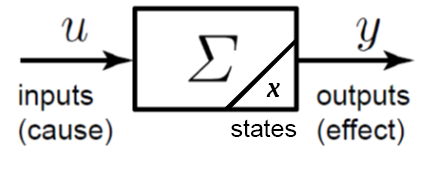
\includegraphics[width=\linewidth]{Signal1}
	\end{multicols*}
	\setlength{\columnseprule}{0.5pt}	
	
	\vspace*{\fill}
	
	\columnbreak
	
	
	\subsection*{Graphical interpretation}
	
	$V=$
	\footnotesize
	\begin{tabular}{rccl}
	&$\underset{\downarrow}{\circ}$&$\underset{\downarrow}{\ast}$\\
	\ldelim[{2}{1mm}&$-0.93$&$-0.36$&\rdelim]{2}{1mm}\\
	&$0.36$&$-0.93$&
	\end{tabular}
	\begin{tabular}{l}
	\\
	$\circ$ will be projected to be $\max(M\cdot u)$.\\
	$\ast$ will be projected to be $\min(M\cdot u)$.
	\end{tabular}
	\normalsize
	
	\mypic{SVDCombined}
		
	\note{
	$M=\begin{bmatrix}1.3&0.1\\1.5&-1\end{bmatrix}\hfill M^T\cdot M = \begin{bmatrix}3.94&-1.37\\-1.37&1.01\end{bmatrix}$
	
	$V=\text{eig}(M^T\cdot M)=\begin{bmatrix}-0.93&-0.36\\0.36&-0.93\end{bmatrix}\hfill U=\text{eig}(M\cdot M^T)$
	
	$M=U\cdot \Sigma \cdot V^T=\begin{bmatrix}-0.55&-0.83\\-0.83&0.55\end{bmatrix}\cdot\begin{bmatrix}2.12&0\\0&0.68\end{bmatrix}\cdot\begin{bmatrix}-0.93&0.36\\-0.36&-0.93\end{bmatrix}$
	}
	
	\begin{itemize}
	\compaq
	\item
	The multiplication of all possible unit vectors $u$ yields the ellipse $Mu$
	\item
	The rows of \hlcyan{$V^T$} contain the unit directions u which are projected on the two semiaxes of $Mu$. ($1_{st}$ row corresponds to $\sigma_{max}$, $2_{nd}$ to $\sigma_{min}$)
	\item
	The columns of $U$ contain the unit directions of the projected u, which multiplied with $\sigma_i$ result in the semiaxes.
	\end{itemize}
	
	\important{\textbf{Identify $V^T$ or $V$ correctly!}}
	
	\subsection*{Singular values of complex matrices}
	
	Norm for complex vectors: 
	
	$||v||^2=\sum\limits_{i=1}^n{a_i^2+b_i^2}=\sum\limits_{i=1}^n{(a_i-jb_i)\cdot(a_i+jb_i)}=\bar{v}^T\cdot v$
	
	\important{$||M||=\sigma_{max}=(M)=\max\limits_i\sqrt{\lambda_i(\bar{M}^T\cdot M)}$}
	
	\note{$\bar{M}^T$ means: transposed and conjugate-complex}
	
	\subsection*{Maximum and minimum gain}
	
	$V$ contains the directions that lead to maximum and minimum output as first and last vertical column.
	
	To find the input signal that leads to maximum gain in the time domain:
	
	\verb+V_max=V(:,1);+
	
	\verb+mu=[abs(V_max(1));abs(V_max(2))];+
	
	\verb+phi=[angle(V_max(1));angel(V_max(2));+
	
	\finn
	
	For the use of $\mu$ and $\phi$ see the next chapter (Frequency response).
	
	\subsubsection{$\sigma_{max}$ , $||\nu||$ and $\max(||y(t)||)$}
	
	If the system is given the input yielding maximum output the following are valid:
	
	\important{$\max(||y(t)||)\leq ||\nu||=\sigma_{max}\cdot||\mu||$}
	
	The same is valid analogously for the minimum output.
	
	\section{Frequency response}
	
	\subsection{Frequency response of SISO systems}
	
	Frequency domain: $Y(s)=P(s)\cdot U(s)$
	
	Time domain, steady state: $y_\infty(t)=\nu\cdot \cos(\omega t-\Psi)\cdot h(t)$
	
	Thus to find the steady state response in the time domain, find $Y(s)$ and determine the phase shift $\Psi$ and the gain $\nu$.
	
	\subsection{Frequency response of MIMO systems}
	
	Time domain:
	
	\footnotesize
	$u(t)=\begin{bmatrix}\mu_1\cdot \cos(\omega t+\phi_1)\cdot h(t)\\
	\mu_2\cdot \cos(\omega t+\phi_2)\cdot h(t)\\
	\vdots\\
	\mu_m\cdot \cos(\omega t+\phi_m)\cdot h(t)\end{bmatrix}\hfill y_\infty(t)=\begin{bmatrix}\nu_1\cdot \cos(\omega t+\psi_1)\cdot h(t)\\
	\nu_2\cdot\cos(\omega t+\psi_2)\cdot h(t)\\
	\vdots\\
	\nu_m\cdot\cos(\omega t+\psi_m)\cdot h(t)\end{bmatrix}$
	\normalsize
	
	\finn
	
	Frequency domain:
	
	$U(s)=e^{\Phi\cdot s/\omega}\cdot\mu\cdot\frac{s}{s^2+\omega^2}\hfill Y_\infty(s)=e^{\Psi\cdot s/\omega}\cdot\nu\cdot\frac{s}{s^2+\omega^2}$
	
	\finn
	
	$\Phi=\text{diag}(\phi_i)\in\mathbb{R}^{m\times m}\hfill \mu=[\mu_1,\mu_2,\ldots,\mu_m]^T\in\mathbb{R}^m$
	
	$\Psi=\text{diag}(\psi_i)\in\mathbb{R}^{m\times m}\hfill \nu=[\nu_1,\nu_2,\ldots,\nu_m]^T\in\mathbb{R}^m$
	
	\important{$y(t)=e^{j\Psi}\cdot\nu=P(j\omega)\cdot e^{j\Phi}\cdot\mu$}

	\small
	\emph{Input and output \textbf{share the same frequency.} $|v|\in (\sigma_{min},\sigma_{max}).$}
	\normalsize

	\finn	
	
	$||P(j\omega)||=\max\limits_{||e^{j\Phi}\mu||}\frac{||e^{j\Psi}\cdot\nu||}{||e^{j\Phi}\cdot\mu||}=\max\limits_{||e^{j\Phi}\cdot\mu||=1}||e^{j\Psi}\cdot\nu||$
	
	\dahe $||e^{j\Phi}\mu||=||\mu||\qquad||e^{j\Psi}\cdot\nu||=||\nu||$
	
	\important{$||P(j\omega)||=\max\limits_{||\mu||}\frac{||\nu||}{||\mu||}=\max\limits_{||\mu||=1}||\nu||$}
	
	Thus we can find an upper and a lower bound to the gain $||\nu||$ using singular value decomposition: ($||\mu||=1$)
	
	\important{$\min\limits_i\sigma_i(P(j\omega))\leq||\nu||\leq\max\limits_i\sigma_i(P(j\omega))$}
	
	\subsection*{Use of the frequency response}
	
	\importname{System norm}{$||G(s)||_\infty=\underset{\omega}{\max}\left(\underset{\omega}{\max}(\sigma_i(G(j\omega))\right)$}
	
	\important{$||G_1(s)\cdot G_2(s)||_\infty\leq||G_1(s)||_\infty\cdot||G_2(s)||_\infty$}
	
	\important{$\mu_{min}=\underset{\omega}{\min}\left(\underset{i}{\min}\ \sigma_i(\mathbb{I}+L(j\omega))\right)$}
	
	\note{$\sigma_i(\ldots)$ \dahe calculate singular values of $\ldots$}
	
	\importname{maximum static error}{$e_\infty=S(0)=\frac{1}{\min\limits_i(\sigma_i(\mathbb{I}+L(j\cdot 0))}$}
	
	\section{Pole placement}
	
	Pole placement is a method to compute a stabilizing controller with certain desired closed loop dynamics.
	
	Depict the closed loop in time domain with two state space models for controller and plant:
	
	\mypic{PolePlacement}
	
	This can be formulated as a single state space model with state variable $\tilde{x}=\begin{pmatrix}x\\z\end{pmatrix}$. Where x is the state variable of the plant and z is the state variable of the controller.
	
	\mypic{PolePlacementOCLoop}
	
	$A_{o/c}=\begin{bmatrix}A&B\cdot H\\\ast&F\end{bmatrix}\qquad \ast=\begin{cases}ol:&0\\cl:&-G\cdot C\end{cases}$
	
	$B_{o/c}=\begin{bmatrix}0\\G\end{bmatrix}\qquad C_{o/c}\begin{bmatrix}C&0\end{bmatrix}$
	
	\finn
	
	\note{$A_{o/c}\element{(nx+nz)}{(nx+nz)}\qquad B_{o/c}\element{(nx+nz)}{ny}$
	
	$C_{o/c}\element{ny}{(nx+nz)}$}
	
	$\lambda(A_{ol})=\lambda(A)\oplus\lambda(F)$
	
	\important{$L_{FSB}(s)=K\cdot(s\cdot I -A)^{-1}\cdot B$}
	
	\important{$D_{FSB}(s)=I+L_{FSB}(s)$}
	
	Challenges:
	\begin{itemize}
	\compaq
	\item What are good locations for the poles?
	\item How to find the controller to place the poles?
	\item No straightforward methodology.
	\item Robustness must be checked a posteriori.
	\end{itemize}
	
	\section{State-feedback regulator}
	
	The state-feedback regulator is defined by a \textbf{static gain}, which allows \textbf{direct placement of the poles}. This approach allows \textbf{no reference tracking}.
	
	\mypic{StateFeedbackRegulator}

	\begin{multicols*}{3}	
	
	\important{$u(t)=-K\cdot x$}
	
	\important{$A_{cl}=A-BK$}	

	$A\element{nx}{nx}$
	
	$B\element{nx}{nu}$
	
	$C\element{ny}{nx}$
	
	$K\element{nu}{nx}$
	
	$Q\element{nx}{nx}$
	
	$R\element{nu}{nu}$
	
	\end{multicols*}
	
	\subsection{Full state feedback: SISO example}
	
	Given:
	
	$\lambda_1=\lambda_2=-5\qquad A=\begin{bmatrix}0&1\\-1&-1\end{bmatrix}\qquad B=\begin{bmatrix}0\\1\end{bmatrix}$
	
	Requested: $K=\begin{bmatrix}k_1&k_2\end{bmatrix}$
	
	\finn	
	
	$\rightarrow\lambda_{1,2}$ are the eigenvalues of $A_{cl}=A-B\cdot K$
	
	Solving the eigenvalue equation: 
	
	$\lambda_{1,2}=-5=-\frac{1+k_2}{2}\pm\frac{\sqrt{(1+k_2)^2-4(1+k_1)}}{2}$
	
	$\rightarrow$ the term under the root must be 0.
	
	\section[LQR]{Linear quadratic regulator (LQR)}
	
	Find a state-feedback regulator such that the objective function J is minimized.
	
	\important{$J(u)=\int_0^\infty{(x(u(t))^T\cdot Q\cdot x(u(t))+u(t)^T\cdot R\cdot u(t)))dt}$}
	
	\note{$Q=\text{diag}(q_i)\element{nx}{nx}\qquad q_i\geq 0\qquad$ i.e. Q is positive definite}
	
	\note{$R=\text{diag}(r_i)\element{nu}{nu}\qquad r_i>0\qquad$ i.e. R is positive semidefinite}
	
	\note{optionally (\hlpink{see below}): $Q=C^T\cdot C$\hfill$R=r\cdot\mathbb{I}^{nu\times nu}$}
	
	\subsection*{Solution}
	
	\important{$u(t)=-K\cdot x(t)\qquad K=R^{-1}\cdot B^T\cdot \Phi$}
	
	Where $\Phi$ is the \hlcyan{only positive definite}, symmetric Solution to the Continuous time Algebraic Riccati Equation (CARE):
	
	\important{$\Phi\cdot B\cdot R^{-1}\cdot B^T \cdot \Phi-\Phi\cdot A-A^T\cdot \Phi-Q=0$}
	
	\important{scalar version: $\frac{1}{r}\cdot B^2\cdot\Phi^2-2\cdot A\cdot\Phi-q=0$}
	
	Matlab: \verb+K=lqr(A,B,Q,R);+
	
	\subsubsection*{Why choose $Q=C^T\cdot C$ ?}
	
	$y=C\cdot x\Rightarrow y^T=x^T\cdot C^T$
	
	$x^T\cdot Q\cdot x=\underbrace{x^T\cdot C^T}_{y^T}\cdot\underbrace{C\cdot x}_{y} = |y|^2$
	
	The resulting objective function J is given by:
	
	\important{$J(u)=\int_0^\infty{||y(u(t))||^2+r\cdot ||u(t)||^2}$}
	
	\subsection*{Prerequisites for successful LQR design}
	
	\importable{1. \{A,B\} & is completly controllable.\\2. \{A,$\bar{C}$\} & is completly observable.$^\ast$}
	
	Where $\bar{C}$ is the full-rank decomposition of the weight Q and is \hlpink{in general independent of C}.
	
	$Q=\bar{C}^T\cdot \bar{C},\bar{C}\in\mathbb{R}^{p\times n}$ where $p=$rank$(Q)\leq n$
	
	Matlab: \verb+C_bar=sqrt(Q)+
	
	$\ast\quad$\hlcyan{Iff Q is chosen such that $Q=\text{diag}(q_i)$,  the second condition is fulfilled automatically.}
	
	\subsection{LQR in the frequency domain}
	
	\important{$L_{LQR}=K\cdot(s\cdot I-A)^{-1}\cdot B$}
	
	\important{$T_{LQR}=C\cdot(s\cdot I-(A-B\cdot K))^{-1}\cdot B$}
	
	\subsection*{Nice to know}
	
	\begin{itemize}
	\compaq
	\item
	Choose r small \dahe \hlcyan{Cheap control}.
	\item
	Choose r big \dahe \hlcyan{Expensive control}.
	\item
	If $R=r\cdot\mathbb{I}_{ny\times ny},r>0\Rightarrow$ good results and 
	
	$\mu_{min}=\underset{\omega}{\min}\left(\underset{i}{\min}\ \sigma_i(\mathbb{I}+L_{LQR}(j\omega))\right)\geq 1$
	\vspace{3pt}
	\item
	LQR guarantees a phase reserve $\phi=\SI{60}{\degree}$ and a minimum return difference of $\mu_{min}=1$.
	\item
	The resulting closed-loop system matrix $A_{cl}=A-B\cdot K$ is a Hurwitz matrix: all its eigenvalues have negative real parts.
	\item
	The resulting controller is not optimal in the sense that it is the best possible one: it is optimal with respect to the given optimization problem.
	\item
	The matrices Q and R are the "tuning knobs" with which the controller properties are influenced in a systematic way. The choice of meaningful weights is not trivial.
	\end{itemize}	
	
	\subsection*{Full state feedback (Pole placement) / LQR}
	
	\small
	\begin{tabular}{p{0.45\linewidth}p{0.45\linewidth}}
	Full state feedback & LQR\\
	Analyse loop gain, simulation results, robustness (MRD). & Analyze loop gain and simulation results. Iterate on weights.\\
	Direct influence on speed of the control system.&\textbf{Guaranteed stability and robustness.}\\
	Unclear how to improve robustness.&Optimal controller w.r.t. chosen weights.\\
	& Indirect tuning of the controller.
	\end{tabular}
	\normalsize
	
	\subsection*{Reference Tracking with LQR}
	
	\mypic{ReferenceLQR}
	
	To introduce reference tracking into LQR a feedforward signal $u_r(t)$ is computed. To keep the controller from fighting the feedforward signal, whilst trying to drive the state $x(t)$ towards the origin, the desired state $x_r(t)$ is subtracted. Thus the controller drives the deviation from the desired state towards zero.
	
	\important{$\underbrace{r(t)\Rightarrow y_r(t)\Rightarrow\begin{cases}u_r(t)\\x_r(t)\end{cases}}_{\text{Requieres advanced methodologies!}}$}
	
	\subsubsection{Simplification: Static reference \& Linear plant}
	\small
	$\begin{matrix}\frac{d}{dt}x(t)=A\cdot x(t)+B\cdot u(t)\\y(t)=C\cdot x(t)=r(t)\end{matrix}\overset{\text{Simplify}}{\Longrightarrow}\begin{matrix}0=A\cdot x_r(t)+B\cdot u_r(t)\\C\cdot x_r(t)=r(t)\end{matrix}$\normalsize
	
	\important{$\begin{bmatrix}x_r(t)\\u_r(t)\end{bmatrix}=\begin{bmatrix}A&B\\C&0\end{bmatrix}^{-1}\begin{bmatrix}0\\r\end{bmatrix}$}
	
	
	
	\section[LQRI]{Extension: LQRI}
	
	\mypic{LQRI}
	
	The LQRI adds an additional output feedback path, where each channel of the control error is integrated. It continues to change its output until the control error is zero. Thus \textbf{reference tracking is possible}.
	
	
	
	\subsection*{Extended LQR}
	
	It is possible to reformulate the problem in order to solve it like an LQR problem.
	
	\mypic{LQRI2}
	
	$\tilde{K}=[K\ \ -K_I]\in\mathbb{R}^{nu\times (nx+ny)}$\hfill$\tilde{x}(t)=\begin{bmatrix}x(t)\\v(t)\end{bmatrix}\in\mathbb{R}^{nx+ny}$
	
	\scriptsize		
	\begin{tabular}{rrrrrrr}
	$\dot{x}(t)=$&$A\cdot x(t)$&$+0\cdot v(t)$&$+B\cdot u(t)$&$+B\cdot w(t)$&$0\cdot r(t)$\\
	$\dot{v}(t)=$&$-C\cdot x(t)$&$+0\cdot v(t)$&$+ 0\cdot u(t)$&$ + 0\cdot w(t)$&$ + \mathbb{I}\cdot r(t)$&$
	$\\
	\vspace{-2ex}\\
	\hline
	\vspace{-2ex}\\
	$\frac{\partial}{\partial t}\tilde{x}(t)=$&$\tilde{A}\cdot \tilde{x}(t)$&&$+\tilde{B}_u\cdot u(t)$&$+\tilde{B}_w\cdot w(t)$&$+\tilde{B}_r\cdot r(t)$	
	\end{tabular}
	\normalsize
	
	\finn
	
	\note{To find L chose $\omega(t)=0$ and $r(t)=0$.}
	
	$\tilde{A}=\begin{bmatrix}A&0\\-C&0\end{bmatrix}\element{nx+ny}{nx+ny}\qquad\tilde{B}=\begin{bmatrix}B\\0\end{bmatrix}\element{nx+ny}{nu}$
	
	\subsubsection{Extension of Q and R}
	
	$\tilde{Q}=\begin{bmatrix}Q&0\\0&\gamma\mathbb{I}\end{bmatrix}\element{nx+ny}{nx+ny}\qquad\tilde{R}=R=r\cdot \mathbb{I}$
	
	\subsubsection{The objective function J}
	
	$\tilde{J}(u)=\int_0^\infty{\cdots+\gamma||v||^2+\cdots dt}$
	
	\columnbreak
	
	\subsection*{Solution}
	
	$u(t)=-\tilde{K}\cdot\tilde{x}(t)=-K\cdot x+K_I\cdot v\qquad \tilde{K}\in\mathbb{R}^{nu\times (nx+ny)}$
	
	\small
	\verb+A_tilde = [A zeros(nx,ny); -C zeros(nx,ny)];+
	
	\verb+B_tilde = [B; zeros(ny,nu)];+
	
	\verb+Q_tilde = [Q zeros(nx,ny); zeros(ny,nx) gamma*eye(ny)]+
	
	\verb+K_tilde=lqr(A_tilde,B_tilde,Q_tilde,R)+
	\normalsize
	
	\finn	
	
	$\tilde{K}=\begin{bmatrix}K&-K_I\end{bmatrix}=\begin{cases}K&=\tilde{K}(:,1:nx)\\K_I&=-\tilde{K}(:,nx+1:nx+ny)\end{cases}$
	
	\note{Syntax to extract K and $K_I$ from $\tilde{K}$ works like that in matlab!}

	\section[Finite Horizon LQR]{Extension: Finite-horizon LQR}
	
	Differences to LQR:
	
	\begin{itemize}
	\compaq
	\item
	The system dynamics can change over time.
	\item
	Finite time horizon means that J, the objective funciont, is integrated only over a finite time span.
	\end{itemize}
	
	\mypic{FiniteHorizonLQR}
	
	\note{$K(t)=\begin{bmatrix}k_1(t)&k_2(t)\end{bmatrix}$}
	
	\section[LQR feedforward]{Extension: LQR feedforward}
	
	\mypic{FeedforwardLQR}
	
	For example we want to calculate the feedforward signal for a locomotive controller.
	
	\subsubsection{Dynamics}
	
	$x=\begin{bmatrix}s\\v\end{bmatrix}\qquad \begin{matrix}s(0)=0\\v(0)=0\end{matrix}\qquad u(t)=F_M(t)$
	
	\subsubsection{Objective function}
	
	$\min \int_0^T{P_{el}(v(t),F_M(t))dt}$
	
	\subsubsection{Constraints}
	
	$|P_{el}(v(t),F_M(t)|<P_{max}\qquad v(t)<v_{max}(s(t))$
	
	$s(T)=s_{END}\qquad v(T)=0$
	
	\section[NOC]{Numerical Optimal Control (NOC)}
	
	The optimal input trajectory $u^*(t\in[0,T])$ is computed numerically for the entire mission and used as feedforward control signal $u_{ff}$.
	
	\begin{center}	
	
	$\underset{\text{Objective}}{\min\limits_{u(t)}J_T\left(x_0,u(t)\right)}=\underset{\text{Stage cost}}{\min\limits_{u(t)}\int_0^T{l\left(x(t),u(t)\right)dt}}+\underset{\text{Terminal cost}}{m\left(x(T)\right)}$
	
	\finn
	
	\begin{equation*}
	\left.
	\begin{aligned}
	\dot{x}(t)&=f\left(t,x(t),u(t)\right)\\
	x(0)&=x_0
	\end{aligned}
	\quad
	\right\}\text{Dynamics}
	\end{equation*}
	
	\finn	
	
	$\underbrace{\underset{\text{state}}{x(t)\in\mathcal{X}},\quad\underset{\text{input}}{u(t)\in\mathcal{U}},\quad \underset{\text{final state}}{x(T)\in\mathcal{X}_f}}_{\text{Constraints}}$
	
	\end{center}
	
	Can be applied to nonlinear dynamics, nonlinear cost functions and constraints can be taken explicitly into account.
	
	
	
	\section[MPC]{Model predictive control (MPC)}
	
	\mypic{ModelPredictiveControl}	
	
	Iterate for every $\Delta t$:
	\begin{enumerate}
	\compaq
	\item
	Measure / Estimate current state: $x(t)=z$
	\item
	Find optimal input trajectory for entire planning window T with NOC. 
	
	\dahe $u^*([0,T]) = \min\limits_{u([0,T])}J_T(z,u([0,T]))$.
	\item
	Implement only the first piece of trajectory. $u^*([0,\Delta t])$
	\end{enumerate}
	
	\small
	\subsection*{Comparison: Classical control / MPC}
	
	\mypic{ClassicalVsMPC}	
	
	\subsubsection{Classical design}
	Dominant issues adressed:
	\begin{itemize}
	\compaq
	\item Disturbance rejection
	\item Noise insensitivity
	\item Model uncertainty
	\end{itemize}
	
	Usually in \textbf{frequency domain}.
	
	\subsubsection{MPC}
	Dominant issues adressed:
	\begin{itemize}
	\compaq
	\item Control constraints (limits)
	\item Process contraints (safety)
	\end{itemize}
	
	Usually in \textbf{time domain} and often with \textbf{discrete time modelling}.
	
	
	\subsection*{MPC features}
	
	\setlength{\columnseprule}{0pt}
	\subsubsection{Pros}
	\begin{multicols*}{2}
	\small
	\begin{itemize}
	\compaq
	\item Any model
	\begin{itemize}
	\compaq
	\item Linear
	\item Nonlinear
	\item Single/multivariable
	\item Time delays
	\item Constraints
	\end{itemize}
	\item Any objective
	\begin{itemize}
	\compaq
	\item Squared error
	\item Absolute error
	\item Worst error over time
	\item Economic objective
	\end{itemize}
	\end{itemize}
	\end{multicols*}
	\setlength{\columnseprule}{0.5pt}
	\subsubsection{Cons}
	\begin{itemize}
	\compaq
	\item Computationally demanding
	\item Stability guarantees?
	\item Feasibility guarantees?
	\item Precise model knowledge necessary
	\item Future external signals known?
	\end{itemize}
	\normalsize
	
	
	
	\section{State observer}
	
	\mypic{StateObserverPrinciple}
	
	The state observer computes an estimate of the state $\hat{x}(t)$ based on the measurement $y(t)$ and the plant input $u(t)$, as well as the model of the plant.
	
	\mypic{StateObserver}
	
	\note{$L_{obs}: \tilde{e}\rightarrow \hat{y}$}
	
	Prerequisites for an ideally working observer:
	\begin{itemize}
	\compaq
	\item Perfectly linear plant
	\item Perfect model
	\item Initial state known
	\item $n_u(t), n_y(t) \equiv 0$
	\end{itemize}	
	
	\dahe In reality this conditions are not fulfilled \dahe Compare $y(t)$ and $\hat{y}(t)$ and feed it back into the observer with the matrix $L\in\mathbb{R}^{nx\times ny}$.
	
	\finn

	observation error: $\bar{x}$	
	
	$\bar{x}(t)=x(t)-\hat{x}(t)\Rightarrow \frac{d}{dt}\bar{x}(t)=\frac{d}{dt}x(t)-\frac{d}{dt}\hat{x}(t)$
	
	$\frac{d}{dt}\bar{x}(t)=Ax+Bu-(\hat{A}x+\hat{B}u+L(y-\hat{y}))$ 
	
	\note{${\hat{A}=A,\hat{B}=B,\hat{C}=C,y=Cx,\hat{y}=C\hat{x}}$}
	
	\important{$\frac{d}{dt}\bar{x}=(A-LC)\bar{x}$}
	
	The eigenvalues of $(A-LC)$ determine the dynamics of the state observation error.
	
	\subsection{Solution (dual LQR problem)}
	
	This problem is similar to the LQR problem solved previously.
	
	$A-L\cdot C \rightarrow (A-L\cdot C)^T=A^T-C^T\cdot L^T$
	
	\finn
	
	\small
	$A-BK\qquad \begin{tabular}{RL}A&\rightarrow A^T\\B&\rightarrow C^T\\Q=\bar{C}^T\cdot \bar{C}&\rightarrow \bar{B}\cdot\bar{B}^T=\text{diag}(b_i)\\R=r\cdot \mathbb{I}&\rightarrow q\cdot \mathbb{I}^{ny}\\K&\rightarrow L^T\end{tabular}\qquad A^T-C^TL^T$\normalsize
	
	\hlcyan{$\bar{B}$ (fictious input matrix) can be chosen to be $B$.}
	
	\important{$L^T=\frac{1}{q}\cdot C \cdot \Psi$}
	
	\important{$\frac{1}{q}\cdot \Psi\cdot C^T\cdot C\cdot \Psi-\Psi\cdot A^T-A\cdot \Psi-\bar{B}\cdot\bar{B}^T=0$}
	
	\note{Where $q$ and $\bar{B}$ are the tuning knobs.}
	
	Matlab: \verb+ L=lqr(A',C',B_bar*B_bar',q*eye(ny))';+
	
	\finn
	
	The speed of the observer is regulated with q. The smaller q the faster the observer and the closer LQG gets to LQR. A faster observer introduces more noise!
	
	\important{$L_{OBS}=C(s\cdot I-A)^{-1}\cdot L\overset{\text{Matlab}}{=}\text{ss}(A,L,C,\text{zeroes}(ny))$}
	
	\subsubsection*{Derivation of $L_{LQR}$ / $L_{OBS}$}
	
	\mypic{DerivationLQG}
	
	\begin{multicols*}{2}
	$\tilde{y}=k\cdot x$
	
	$\dot{x}=A\cdot x+B\cdot \tilde{e}$
	
	$s\cdot X=A\cdot X+B\cdot\tilde{E}$
	
	$(s\cdot\mathbb{I}-A)\cdot X=B\cdot\tilde{E}$
	
	$X=(s\cdot\mathbb{I}-A)^{-1}\cdot B\cdot\tilde{E}$
	
	\important{$L_{LQR}=K(s\cdot\mathbb{I}-A)^{-1}\cdot B$}
	
	\columnbreak
	
	$\tilde{y}=C\cdot \hat{x}$
	
	$\hat{\dot{x}}=A\cdot\hat{x}+L\cdot\tilde{e}$
	
	$\tilde{y}=C(s\cdot\mathbb{I}-A)^{-1}\cdot L\cdot\tilde{E}$
	
	\important{$L_{OBS}=C\cdot(s\cdot\mathbb{I}-A)^{-1}\cdot L$}
	
	\end{multicols*}
	
	\subsubsection*{SS Model of observer including LQR (K-matrix)}
	
	\begin{tabular}{l@{ = }l@{$\qquad$}l}
	\verb+A_o+&\verb+A-BK-LC+\\
	\verb+B_o+&\verb+-L+\\
	\verb+C_o+&\verb+eye(nx)+& use \verb+eye+ to output all states\\
	\verb+D_o+&\verb+zeros(ny,nu)+
	\end{tabular}

	\subsection{Kalman filter}
	
	Kalman filters have the same structure as state observers. If the disturbance and the noise are Gaussian zero mean white noise signals, they allow finding an optimal observer design.
	
	$L_K=lqr(A',C',B*R_u*B',R_y)';$
	
	\note{$R_u$ and $R_y$ are the auto-covariance matrices of the disturbance and the noise signal, respectively.}
	
	Kalman filters are widely used, because they represent a straightforward solution to the problem of sensor fusion, in which the information provided by several sensor measuring different physical variables are to be combined in a meaningful way.

	\section[LQG]{Output feedback controller (LQG)}

	\note{LQG = Linear quadratic Gaussian}
	
	LQG is the connection of the LQR gain K, that previously relied on state feedback, with a state observer. Thus now only the output $y(t)$ is used which is necessary since realistically the state variables are not available.
	
	\mypic{LQGAdditional}	
	
	\mypic{LQG}
	
	\subsection*{State-space matrices, Controller}	
	
	$A_c=A-B\cdot K-L\cdot C\element{nx}{nx}$
	
	$B_c=-L\element{nx}{ny}$
	
	$C_c=-K\element{nu}{nx}$
	
	$D_c=0\element{ny}{nu}$
	
	\subsection*{State-space matrices, open loop (L) / closed loop (T)}
	
	$\tilde{x}(t)=\begin{bmatrix}x(t)\\ \hat{x}(t)\end{bmatrix} \qquad\begin{matrix}\text{State of the plant}\\ \text{State of the controller}\end{matrix}$
	
	\small
	$A_{ol/cl}=\begin{bmatrix}A&-BK\\ \ast&A-BK-LC\end{bmatrix}$\hfill$\ast=\begin{cases}0\element{nx}{nx}&\text{L(s): } e\rightarrow y\\LC&\text{T(s): }r\rightarrow y\end{cases}$
	
	$B_{ol/cl}=\begin{bmatrix}0\element{nx}{ny}\\-L\end{bmatrix}$\hfill$C_{ol/cl}=\begin{bmatrix}C&0\element{ny}{nx}\end{bmatrix}$
	
	$D_{ol/cl}=\element{ny}{nu}$	
	\normalsize
	
	\subsection*{Stability}
	
	For the analysis of the stability of the LQG closed loop system, the eigenvalues of $A_{cl}$ need to be analyzed.
	
	$A_{cl}=\begin{bmatrix}A&-B\cdot K\\L\cdot C&A-B\cdot K -L\cdot C\end{bmatrix}$
	
	$T=\begin{bmatrix}I_{n\times n}&0_{n\times n}\\I_{n\times n}&-I_{n\times n}\end{bmatrix}$ Transforms A, not changing EV's
	
	$T^{-1}\cdot \tilde{A}_{cl}\cdot T = \begin{bmatrix}A-B\cdot K & B\cdot K\\0_{n\times n}&A-L\cdot C\end{bmatrix}$
	
	\finn
	
	\hlcyan{\textbf{The EV's of the LQG closed loop are the combination of $A-B\cdot K$ and $A-L\cdot C$.}}
	
	\important{LQG inherits stability but not robustness.}
	
	\note{See LTR for the robustness of LQG.}
	
	\section[LTR]{Loop transfer recovery (LTR)}
	
	The guaranteed robustness properties of the LQR have been lost for the LQG control loop. \hlcyan{Loop transfer recovery is a method (not a controller)} to \glqq recover\grqq as much of this robustness as possible.
	
	\mypic{LoopTransferRecovery}
	
	\subsection*{Standard LQG/LTR recipe ($nu\geq ny$)}
	
	\begin{enumerate}[leftmargin=*]
	\compaq
	\item
	Plant modelling
	\item
	Linearization, Nomralization
	\item
	Plant extension with I-part. Use extended plant only for state feedback, not for observer.
	\item
	Definition of specification in frequency domain.
	\item
	Derive loop shaping state observer.
		
	\begin{enumerate}[leftmargin=*]
	\compaq
	\item
	\verb+Psi=care(A',C',B_bar*B_bar',beta*q*eye(ny)+	
	\item

	\verb+L=(1/q*C*Psi)'+

	
	\item
	Find $\bar{B}\cdot\bar{B}'\in\mathbb{R}^{n\times n}$,$q>0$ and $\beta\geq 1$, which fulfill specifications with a $\sim$3dB margin
	\item
	$L_{obs}(s)=C\cdot(s\cdot I-A)^{-1}\cdot L$
	\end{enumerate}
	\item 
	\hlcyan{Derive LTR state feedback regulator}
	\begin{enumerate}[leftmargin=*]
	\compaq
	\item
	\verb+K=lqr(A,B,C'*Q_y*C,rho*R_u)+
	\item
	Find $Q_y\in\mathbb{R}^{ny\times ny}$ and $R_u\in\mathbb{R}^{nu\times nu}$ (often $Q_y=\mathbb{I}^{ny\times ny}$ and $R_u = \mathbb{I}^{nu\times nu}$
	\item Decrease rho until requirements are satisfied
	\item \footnotesize $L_{LTR}(s)=C\cdot(s\cdot I-A)^{-1}\cdot B\cdot K\cdot (s\cdot I-(A-B\cdot K-L\cdot C))^{-1}\cdot L$\normalsize
	\end{enumerate}
	\item
	Controller realization
	\end{enumerate}
	
	\mypic{LTRSpecifications}
	
	\subsection*{Dual LQG/LTR recipe ($ny\geq nu$)}
	
	\begin{enumerate}
	\compaq
	\setcounter{enumi}{4}
	\item
	Derive loop shaping LQ regulator
	
	
	\begin{enumerate}[leftmargin=*]
	\compaq
	\item
	\verb+Phi=care(A,B,Q,beta*r*eye(nu))+
	
	\item
	\verb+K=1/r*B'*Phi+
	\item
	Find $Q\in\mathbb{R}^{n\times n}$, $r>0$ and $\beta \geq 1$, which fulfill specifications with a $\sim$3dB margin
	\item $L_{LQR}(s)=K\cdot(s\cdot I-A)^{-1}\cdot B$
	\end{enumerate}
	\item
	\hlcyan{Derive LTR observer}
	\begin{enumerate}[leftmargin=*]
	\compaq
	\item
	\verb+L=lqr(A',C',B*Q_u*B',mu*R_y)'+
	\item 
	Find $Q_u\element{nu}{nu}$, $R_y\in\mathbb{R}^{ny\times ny}$ 
	
	(often $Q_u=\mathbb{I}^{nu\times nu}$ and $R_y=\mathbb{I}^{ny\times ny})$
	\item
	Decrease $mu$ until requirements are satiesfied
	\item
	$L_{LTR}(s)=C\cdot(s\cdot I-A)^{-1}B\cdot K\cdot (s\cdot I-(A-B\cdot K-L\cdot C))^{-1}\cdot L$
	\end{enumerate}
	\end{enumerate}
	
	\subsection*{Short Summary}
	
	\subsubsection*{Standard LTR ($nu\geq ny$)}
	
	\begin{itemize}	
	\compaq
	\item
	Design a robust observer with any method (preferably with LQR, the weight $q\cdot\mathbb{I}$ and $\beta>1$).
	\item
	Compute the LTR regulator (see LTR recipe point 6) with weights $Q=C^T\cdot C$ and $\rho\cdot \mathbb{I}$.
	\item
	With $\rho\rightarrow 0$, the LQG loop gain approaches the loop gain of the observer.
	\end{itemize}
	
	\subsubsection*{Dual LTR ($ny\geq nu$)}
	
	\begin{itemize}
	\compaq
	\item
	Design a robust LQ regulator with any method (preferably with LQR, the weight $r\cdot\mathbb{I}$ and $\beta>1$).
	\item
	Compute the LTR observer (see LTR recipe point 6) with weights $\bar{B}\cdot\bar{B}^T=B\cdot B^T$ and $\mu\cdot\mathbb{I}$.
	\item
	With $\mu\rightarrow 0$ the LQG loop gain approaches the loop gain of the LQ regulator.
	\end{itemize}	
	
	\section{LQG Extensions}
	
	\subsection{LQG reference tracking}
	
	\dahe static feedforward gain
	
	\note{LQG is not well suited for reference tracking because the change in r(t) introduces an observer error and yields a static control error.}	
	
	\mypic{LQGReference}
	
	$\Lambda=$\hlpink{L}$+B\cdot\Gamma\qquad\Gamma=-\left(\tilde{C}\cdot\tilde{A}_{cl}^{-1}\cdot\tilde{B}_r\right)^{-1}$
	
	\note{\hlpink{because $-L\cdot r$ is added it has to be removed again by $\Lambda$ to avoid an observer error (LQG was designed with r=0).}}
	
	$\Gamma$ is chosen such that the static gain from r\dahe y is equal to 1.	
	
	\mypic{LQGReference2}
	
	$\tilde{A}_{cl}=\begin{bmatrix}A&-B\cdot K\\L\cdot C&A-B\cdot K-L\cdot C\end{bmatrix}\qquad\tilde{B}_r=\begin{bmatrix}B\\B\end{bmatrix}\qquad \tilde{C}=\begin{bmatrix}C&0\end{bmatrix}$
	
	\mypic{LQGReferenceSimulink}
	
	\subsection{LQGI}
	
	\mypic{LQGI}
	
	\finn
	
	\note{without FF:}
	
	$\begin{bmatrix}\dot{\hat{x}}\\\dot{v}\end{bmatrix}=\begin{bmatrix}A-B\cdot K-L\cdot C&B\cdot K_I\\0&0\end{bmatrix}\cdot\begin{bmatrix}\hat{x}\\v\end{bmatrix}+\begin{bmatrix}-L\\I\end{bmatrix}e$
	
	$u=\begin{bmatrix}-K&K_I\end{bmatrix}\cdot\begin{bmatrix}\hat{x}\\v\end{bmatrix}$	
	
	\mypic{LQRISimulink}
	
	\subsubsection{Design procedure}
	
	\begin{enumerate}
	\compaq
	\item
	Form the extended system $\{\tilde{A},\tilde{B},\tilde{C}\}$ \hlcyan{\textbf{(see LQRI)}}. From that find $\tilde{K}=\begin{bmatrix}K,-K_I\end{bmatrix}$. Start with simple weights $(R=r\cdot I, \text{etc.})$ and iterate on $r$ and $\gamma$ until the desired system behaviour is achieved.
	\item
	Design an observer gain L for the original system $\{A,B,C\}$ \textbf{(see state observer)}
	\item
	Optionally add a feed forward. $\Gamma = \mathbb{I}$, since the closed loop feedback system has a static gain of $\mathbb{I}$ and $\Lambda = L + B$.
	\end{enumerate}
	
	\section{$\beta$ Method}
	
	The minimum return difference of the LQR state feedback regulator and the state observer are guaranteed to be 1, if $R=r\cdot I$, $Q=q\cdot I$ respectively.
	
	\mypic{BetaMethod}
	
	Thus $L(j\omega)$ shall not enter the inner circle with radius 1. This radius can not be increased as such, since the loop gain of any stable system converges to the origin.
	
	The $\beta$ method allows to further increase the robustness by shifting the circle towards the left while increasing its radius. \textbf{Resonable values for $\beta$: between 2 and 5.}
	
	\subsection*{State feedback regulator}
	
	$\frac{1}{r\cdot\beta}\cdot\Phi\cdot B\cdot B^T\cdot\Phi-\Phi\cdot A-A^T\cdot\Phi-Q=0$
	
	$K=\frac{1}{r}\cdot B^T\cdot \Phi$
	
	\verb+Phi = care(A,B,Q,beta*r*eye(nu))+

	\verb+K=1/(r*B'*Phi)+
	
	\subsection*{State observer}
	
	$\frac{1}{q\cdot\beta}\cdot\Psi\cdot C^T\cdot C \cdot\Psi-\Psi\cdot A^T-A\cdot\Psi-\bar{B}\cdot\bar{B}^T=0 $
	
	$L^T=\frac{1}{q}\cdot C \cdot \Psi$
	
	\verb+Psi=care(A',C',B_bar* B_bar',beta*q*eye(ny))+
	
	\verb+L=(1/q*C*Psi)'+

	\part{Appendix}
	
	\section{MATLAB}
	
	\small
	\begin{tabular}{p{0.5\linewidth}p{0.4\linewidth}}
	\hline
	\multicolumn{2}{c}{Basics}\\
	\hline
	\hline
	Struct\\
	\hline
	\verb+parvec(1).a=...+\\
	\verb+parvec(1).b=...+\\
	\verb+parvec(1).c=...+\\
	\verb+parvec(2).a=...+\\
	$\vdots$&\\
	\verb+parvec(3).c=...+\\
	\verb+for i=1:length(parvec)+\\
	\verb+  a=parvec(i).a+\\
	\verb+  b=parvec(i).b+\\
	\verb+  c=parvec(i).c+\\
	\verb+end+&\\
	\end{tabular}
	\begin{tabular}{p{0.5\linewidth}p{0.4\linewidth}}
	\hline
	Matrix / Vector\\
	\hline
	Matrix P(3x3)\\
	\verb+v=P(:,1)+&first column (Spalte)\\
	\verb+v=P(1,:)+&first row (Zeile)\\
	Matrix A(2x3)\\
	\verb+size(A,1)=2+&\verb+size(A,2)=3+
	\end{tabular}
	\begin{tabular}{p{0.37\linewidth}p{0.53\linewidth}}
	\hline
	\multicolumn{2}{c}{Systems}\\
	\hline
	\hline
	\verb+s=tf('s')+&\dahe sys=P(s)\\
	\verb+sys=tf(num,den)+&\begin{tabular}{l}num=$b_m,\ldots ,b_0	]$\\den$=[a_n,\ldots,a_0]$\end{tabular}\\
	\verb+sys=zpk([Z],[Pi],k_p)+&NST,Pole,Gain\\
	\verb+sys=ss(A,b,c,d)+&state-space-model\\
	\verb+tf(sys)+&Find transfer function of a system\\
	\verb+sys.iodelay=time+& Add a delay to a system\\
	\verb+T=feedback(L,1)+&T$\qquad$ MIMO: 1\dahe eye\\
	\verb+S=feedback(1,L)+&S$\qquad$ MIMO: 1\dahe eye\\
	\verb+L=series(C,P)+&L\\
	\verb|P=C*(s*I-A)^(-1)*B+D|&MIMO TF\\
	\verb+X=Loopsens(P,C)+&\verb+X.Li=Lu+$\quad$\verb+X.Lo=Le+\\
	\verb+minreal(sys)+&Minimal realization\\
	\hline
	\end{tabular}
	\begin{tabular}{p{0.5\linewidth}p{0.4\linewidth}}
	\multicolumn{2}{c}{Analysis}\\
	\hline
	\hline
	\verb+step(sys)+&step response of system\\
	\verb+[Gm,Pm,Wcg,Wcp]=margin(L)+&\begin{tabular}{ll}GM &= gain margin\\PM&=phase margin\\Wcg&=crossover frequency\\Wcp&= critical phase fr. \end{tabular}\\
	&$k_{p,krit}=GM$\\
	\verb+[mag,pha,omegaout]=bode(sys)+&Get bodeplot-data\\
	\verb+[mag,pha]=bode(sys,omega)+&Get bodeplot-point\\
	\verb+omega=logspace(a,b,n)+& n points $\in$ decades a,b\\
	\verb+pole(sys)+ & Calculate poles of sys\\
	\verb+zero(sys)+ & Calculate zeros of sys\\
	\verb+[V,D]= eig(A)+ & Eigenvectors (V) and -values (D)\\
	\verb+D=eig(A)+& Eigenvalues of A\\
	\verb+rank(A)+ & Rank of A\\
	\verb+crtb(sys), crtb(A,b)+&Controllability matrix\\
	\verb+obsv(sys), obsv(A,c)+&Observability matrix\\
	\verb|min(abs(bode(1+L)))|&$\mu_{min}$ SISO\\
	\verb+SV=sigma(sys,omega)+&extract singular values\\
	\verb+RGA=P.*P.'^-1+&RGA for $P\in\mathbb{C}^{n\times n}$\\
	\verb+RGA=P.*pinv(P).'+&RGA for $P\in\mathbb{C}^{n\times m}$\\
	\verb+P=evalfr(SS,omega)+&P($j\omega$)\\
	\end{tabular}
	\begin{tabular}{p{0.5\linewidth}p{0.4\linewidth}}
	\verb+[U S V]=svd(P)+&Singular value decomposition\\
	\verb+V_max=V(:,1)+&Direction of maximum gain\\
	\verb+mag2db(y)+&Convert magnitude to dB\\
	\verb+db2mag(dB)+&Convert db to magnitude\\
	\verb+mu=[abs(V_max(1));abs(V_max(2))];+\\
	\verb+phi=[angle(V_max(1));angel(V_max(2));+
	\end{tabular}
	\begin{tabular}{p{0.4\linewidth}p{0.5\linewidth}}
	\hline
	\multicolumn{2}{c}{Diagrams}\\
	\hline
	\hline
	\verb+subplot(x,y,n)+&x rows, y columns, nth plot\\
	\verb+hold on+&not overwrite plots\\
	\verb+xlabel('Time [s]')+&Label x-axis\\
	\verb+bode(sys)+&Bode diagram\\
	\verb+margin(sys)+&Bode diagram with Gm and Pm\\
	\verb+nyquist(sys)+&Nyquist plot\\
	\verb+bodemag(sys)+&Only plot magnitude\\
	\verb+impulse(sys)+&impulse answer\\
	\verb+step(sys)+&step answer\\
	\verb+P=evalfr(sys,i*freq)+&$P(j\omega)|_{\omega=freq}$\\
	\verb+omega=logspace(a,b,n)+&$w(i)\in[10^a,10^b], n=length(w)$\\
	\verb+sigma(sys)+&singular value plot\\
	\verb+semilogx(Y)+&logarithmic scale on X-axis, linear scale for Y-axis\\
	\verb+semilogy(X)+&\\
	\verb+loglog(X)+&double logarithmic plot\\
	\verb+squeeze(A)+&Remove singleton dimensions\\
	\end{tabular}
	\normalsize
	
	\section{Complex numbers}
	
	\begin{center}
	$a+i\cdot b=|a+i\cdot b|\cdot e^{i\cdot\angle(a+i\cdot b)}$

	\finn
	
	$\left|\frac{a+i\cdot b}{c+i\cdot d}\right|=\sqrt{\frac{a^2+b^2}{c^2+d^2}}$

	\finn
	
	$\angle\left(\frac{a+i\cdot b}{c+i\cdot d}\right)=\arctan\left(\frac{b}{a}\right)-\arctan\left(\frac{d}{c}\right)$
	\end{center}
	
	\section{Trigonometric functions}
	
	\begin{center}
	\begin{tabular}{lccccccc}
	\hline
	\hline
	$\alpha[^\circ]$&0&30&45&60&90&120&180\\
	$\alpha[rad]$&0&$\frac{\pi}{6}$&$\frac{\pi}{4}$&$\frac{\pi}{3}$&$\frac{\pi}{2}$&$\frac{2\pi}{3}$&$\pi$\\
	\hline
	$\sin(\alpha)$&0&$\frac{1}{2}$&$\frac{\sqrt{2}}{2}$&$\frac{\sqrt{3}}{2}$&$1$&$\frac{\sqrt{3}}{2}$&0\\
	$\cos(\alpha)$&1&$\frac{\sqrt{3}}{2}$&$\frac{\sqrt{2}}{2}$&$\frac{1}{2}$&0&$-\frac{1}{2}$&-1\\
	$\tan(\alpha)$&0&$\frac{\sqrt{3}}{3}$&1&$\sqrt{3}$&$\pm\infty$&$-\sqrt{3}$&0\\
	$\cot(\alpha)$&$\pm\infty$&$\sqrt{3}$&1&$\frac{\sqrt{3}}{2}$&0&$-\frac{\sqrt{3}}{2}$&$\pm\infty$\\
	\hline
	\hline
	\end{tabular}
	\end{center}
	
	\section{Euler identities}
	
	\begin{center}
	$\sin(x)=\frac{1}{2i}(e^{ix}-e^{-ix})$
	
	\finn
	
	$\cos(x)=\frac{1}{2}(e^{ix}+e^{-ix})$
	
	\finn
	
	$e^{ix}=\cos(x)+i\cdot\sin(x)$
	
	\section{dB}
	
	\begin{tabular}{l|llllllll}
	\hline
	Value&0.01&0.1&0.5&$\frac{1}{\sqrt{2}}$&1&$\sqrt{2}$&2&10\\
	dB&-40&-20&-6&-3&0&3&6&20\\
	\hline
	\end{tabular}
	
	\finn
	
	$[dB]=20\cdot\log_{10}{X}$\hfill$X=10^{\frac{dB}{20}}$\hfill$\frac{1}{X}|_{dB}=-X|_{dB}$
	
	\end{center}
	
	\vspace{3ex}
	
	\setlength{\columnseprule}{0pt}
	\small
	\begin{multicols*}{2}
	\begin{tabular}{ll@{=}l}
	number of states&n&nx\\
	number of inputs&m&nu\\
	number of outputs&p&ny\\
	\end{tabular}
	\normalsize
	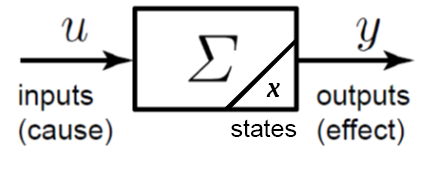
\includegraphics[width=\linewidth]{Signal1}
	\end{multicols*}
	\setlength{\columnseprule}{0.5pt}
	
\end{multicols*}

\mypic{MatlabAddition}

\mypic{Appendix1}

\mypic{Appendix2}

\mypic{Appendix3}

\mypic{Appendix4}

\mypic{Appendix5}

\end{document}

























